\documentclass{ta-its}
\usepackage{hyperref}
\usepackage{cleveref}
\usepackage{nameref}
\usepackage{multirow}
\usepackage{graphicx}
\usepackage{array}
\usepackage{tabularx}
\usepackage{tabulary}
\usepackage{lmodern}  
\usepackage{etoolbox}
\usepackage{listings}
%\usepackage{longtable}
%\usepackage{algorithm} 
\usepackage{float}
\usepackage{slantsc}
\usepackage{booktabs}% http://ctan.org/pkg/booktabs
\usepackage[noend]{algpseudocode}
\usepackage{caption}
\usepackage{subcaption}
\usepackage{amsmath}
\usepackage{colortbl}
%\usepackage{pgfplots}
%\usepackage{tikz}
\usepackage{ltxtable} %for long table
% \usepackage{lon} %for long table
\captionsetup[ltxtable]{position=bottom}
\captionsetup[table]{position=bottom}

\usepackage{lipsum} %for lorem ipsum
\usepackage{blindtext} %for lorem ipsum

\usepackage{xcolor} %start packages for colored code listing
\usepackage{upquote} %start packages for colored code listing
\def\plaintext{\textit{plain text }}
\def\ciphertext{\textit{ciphertext }}
\usepackage{enumitem} % for advanced enumerate numberings
\usepackage{scrextend}
% \usepackage{apacite} % for APA citing style

\usepackage[autostyle]{csquotes}
\usepackage{babel}
\usepackage{wrapfig} %untuk wrapfigure?

\usepackage{lscape} %untuk landscape di bagian-bagian tertentu

\newcommand{\mychapter}[2]{
    \setcounter{chapter}{#1}
    \setcounter{section}{0}
    \chapter*{#2}
    \addcontentsline{toc}{chapter}{#2}
}

\newcommand{\mylipsum}
{Dolore blandit mus ultricies justo ultrices, a vel wisi aenean integer lacus vitae, metus lorem nulla, tempor sed odio lacus sit nostra.}

\newcommand{\indentenum}{
    \hspace{\labelwidth}\phantom{\texttt{type}-}
}


\renewcommand{\lstlistingname}{Kode Sumber}
\renewcommand{\lstlistlistingname}{DAFTAR KODE SUMBER}

\definecolor{listinggray}{gray}{0.9}
%\definecolor{lbcolor}{rgb}{0.9,0.9,0.9}
\lstset{
%backgroundcolor=\color{lbcolor},
    tabsize=4,    
%   rulecolor=,
    language=[GNU]C++,
        basicstyle=\scriptsize,
        upquote=true,
        aboveskip={1.5\baselineskip},
        columns=fixed,
        showstringspaces=false,
        extendedchars=false,
        breaklines=true,
        prebreak = \raisebox{0ex}[0ex][0ex]{\ensuremath{\hookleftarrow}},
        frame=single,
        numbers=left,
        showtabs=false,
        showspaces=false,
        showstringspaces=false,
        identifierstyle=\ttfamily,
        keywordstyle=\color[rgb]{0,0,1},
        commentstyle=\color[rgb]{0.026,0.112,0.095},
        stringstyle=\color[rgb]{0.627,0.126,0.941},
        numberstyle=\color[rgb]{0.205, 0.142, 0.73},
%        \lstdefinestyle{C++}{language=C++,style=numbers}’.
}
\lstset{
    %backgroundcolor=\color{lbcolor},
    tabsize=4,
  language=C++,
  captionpos=b,
  tabsize=3,
  frame=lines,
  numbers=left,
  numberstyle=\tiny,
  numbersep=5pt,
  breaklines=true,
  showstringspaces=false,
  basicstyle=\footnotesize,
%  identifierstyle=\color{magenta},
  keywordstyle=\color[rgb]{0,0,1},
  commentstyle=\color{Darkgreen},
  stringstyle=\color{red}
  }
  
 %formatting code sources
\newlist{inlinelist}{enumerate*}{1}
\setlist*[inlinelist,1]{
	label={\alph*)},font={\color{red!50!black}\bfseries}
} %enumerate?

\makeatletter
\def\l@lstlisting#1#2{\@dottedtocline{1}{1.5em}{3em}{#1}{#2}}
\makeatother
%\counterwithin*{equation}{chapter}
\raggedbottom

\title{Optimasi Kasiski Examination pada Studi Kasus SPOJ The Bytelandian Cryptographer (Act IV)}{Optimization Kasiski Examination on Study Case SPOJ The Bytelandian Cryptographer (Act IV)}{KI141502} 

% \author{Nama Lengkap}{NRP}
\author{Freddy Hermawan Yuwono}{5113100040}

% \supervisorOne{Nama Pembimbing Satu}{NIP}
% \supervisorTwo{Nama Pembimbing Dua}{NIP}
\supervisorOne{Rully Soelaiman, S.Kom, M.Kom}{197002131994021001}
\supervisorTwo{Wijayanti Nurul Khotimah, S.Kom., M.Sc}{198603122012122004}

% \degree{Nama Gelar}{Bidang Studi}{Program Studi}{Jurusan}{Jurusan (English)}{Fakultas}{Fakultas Singkatan}{Fakultas (English)}
\degree{Sarjana Komputer}{Algoritma Pemrograman}{S1}{Teknik Informatika}{Informatics}{Teknologi Informasi}{FTIf}{Information Technology}

% \time{bulan}{tahun}
\time{Desember}{2017}


\begin{document}
    \maketitle
%    \pagenumbering{}
	\pagenumbering{roman}
    \legalityPaper
    \begin{abstrak}
		\indent Pada era digitalisasi ini, tingkat kebutuhan masyarakat akan informasi semakin meningkat. Hal ini menyebabkan pertukaran informasi menjadi sangat mudah. Hal ini membuat informasi yang bersifat sensitif dapat terjadi kebocoran informasi kepada pihak - pihak yang tidak berkepentingan. Kebocoran informasi terbagi menjadi dua apabila dilihat dari keutuhan informasi yang didapat, yaitu sebagian dan seutuhnya. Kebocoran informasi yang bersifat sebagian, membuat pihak-pihak yang tidak berkepentingan tetapi yang menginginkan informasi tersebut, berusaha untuk mendapatkan informasi yang utuh dari potongan-potongan informasi yang telah didapatkan. 
\\
\indent Permasalahan dalam buku tugas akhir ini adalah permasalahan untuk mendapatkan \textit{plaintext} sebanyak-banyaknya dari \textit{ciphertext} dan batas atas panjang kunci pada metode enskripsi yang menggunakan teknik \textit{Vigenere Cipher}. Dalam permasalahan ini diberikan \textit{plaintext} dan \textit{ciphertext}, akan tetapi terdapat informasi yang hilang pada keduanya. Diberikan batas atas panjang kunci, dimana batas atas ini belum tentu panjang kunci yang sesungguhnya. Untuk dapat merekonstruksi \plaintext dari kepingan informasi yang didapatkan diperlukan untuk mencari panjang kunci yang di dapatkan dengan cara memodifikasi \textit{Kasiski Examination} dan \textit{Intersection}. Beberapa hal yang perlu diperhatikan seperti mempercepat dari \textit{Kasiski Examination} dan juga \textit{Intersection} terhadap hasil yang diperoleh dari pencarian panjang kunci.
\\  
\indent Hasil dari tugas akhir ini telah berhasil untuk menyelesaikan permasalahan yang telah diangkat dengan benar. Waktu yang diperlukan untuk dapat menyelesaikan masukan sebesar 2MB dalam 4,42 detik dengan alokasi memori sebesari 26,5MB.
\\
\noindent \textbf{Kata-Kunci}:  \textit{Ciphertext}, \textit{Kasiski Examination}, \textit{Optimisasi},\textit{Plaintext}.
\end{abstrak}



    \begin{abstract}
	\indent In this Digitalization era, the level of community needs for information is increasing. This make exchanging the information very easy. This makes the sensitive information leakage to the unauthorized party. The leakage of information divided into 2 when viewed from the integrity of information they get. First they get all information or second they only get a partial of information. Partial information leakage, make unauthorized party to reconstruct the information they get from all piece information they have already obtain.
\\
\indent The problem in this undergraduate thesis book is the problem to get plaintext as much as possible from the ciphertext and upper bound of key length. The encryption method is using the Vigenere Cipher technique. Given the plaintext and ciphertext, but there is missing information in both of them. Given the upper bound of key length, that is not real key length. To reconstruct plaintext from piece information, must find the length of key from modify Kasiski Examination and Intersection. Some things to note that using only modify Kasiski Examination and Intersection can not solving the problem. Required to optimize both of them to get the answer and right time.
\\
\indent The results show that this problem is successfully solved. Averaging time of 4.42 second and averaging memory use about 26.5MB to solve 2MB data.
\\
\noindent \textbf{Keywords}: \textit{Plaintext}, \textit{Ciphertext}, \textit{Kasiski Examination},  \textit{Optimization}.
\end{abstract}
    \mychapter{0}{KATA PENGANTAR}
    
	  Puji Syukur kepada Tuhan yang Maha Esa, atas berkatNya penulis dapat menyelesaikan buku berjudul \textbf{\judul}. 
	  \newline
	  \indent Selain itu, pada kesempatan ini penulis menghaturkan terima kasih sebesar-besarnya kepada pihak-pihak yang tanpa mereka, penulis tidak akan dapat menyelesaikan buku ini:
  \begin{enumerate}
  	\item \textbf{\textit{Tuhan Yesus Kristus}} atas segala berkat, limpahan karunia, kesempatan, dan rancangan-Nya penulis masih diberi nafas kehidupan, waktu, tenaga dan pikiran untuk menyelesaikan buku ini.
    \item \textbf{Alm. Papa} yang selalu menguatkan, menasehati, dan luar biasa sabar dalam mengingatkan penulis agar tidak lupa menjaga kesehatan dan selalu bersyukur selama masa studi.
    \item \textbf{Mama dan saudara} yang selalu memberikan saran, dukungan, doa dan tidak lupa untuk selalu bersyukur selama masa studi.
    \item \textbf{Yth. Bapak Rully Soelaiman} sebagai dosen pembimbing I yang telah banyak memberikan ilmu, bimbingan, nasihat, motivasi, serta waktu diskusi sehingga penulis dapat menyelesaikan tugas akhir ini; dan \\
	    \textbf{Yth. Ibu Wijayanti Nurul Khotimah} sebagai dosen pembimbing II yang memberi bimbingan, saran teknis dan administratif, diskusi dan pemecahan masalah dalam pembuatan dan penulisan buku tugas akhir.
    \item \textbf{Teman-teman Sarjana Komedi} yang telah mengingatkan, memberikan semangat dan inspirasi untuk terus melanjutkan tugas akhir di saat penulis kehilangan semangat.
    \item \textbf{Teman-teman S1 Teknik Informatika 2013} yang membantu, menyemangati dan bertukar pikiran dengan  penulis selama pengerjaan tugas akhir ini.
    \item \textbf{Teman-teman S1 Teknik Informatika bukan 2013}, yang telah banyak membantu, menyemangati dan bertukar pikiran dengan penulis selama pengerjaan tugas akhir ini, terutama pada Steven, Theo, Daniel, dan Glenn.
    \item Serta semua pihak yang tidak tertulis, baik yang membantu dalam proses pengujian, membantu memikir saat ada masalah, dan lainnya yang telah turut membantu penulis dalam menyelesaikan Tugas Akhir ini.
  \end{enumerate}
  
  \indent Penulis menyadari bahwa Tugas Akhir ini masih memiliki banyak kekurangan. Oleh karena itu, penulis berharap kritik dan saran dari pembaca sekalian untuk memperbaiki buku ini ke depannya. Semoga tugas akhir ini dapat memberikan manfaat yang sebaik-baiknya.

  \hfill Surabaya, Januari 2018 \\ \\ 


  \hfill Freddy Hermawan Yuwono

\cleardoublepage % Mengisi penanda halaman genap yang kosong


    \tableofcontents % Daftar isi
    \listoftables % Daftar tabel
    \listoffigures % Daftar gambar
    \lstlistoflistings % Daftar Kode Sumber

  \mainmatter % Halaman utama, dengan judul BAB X
    \chapter{PENDAHULUAN}
  Pada bab ini akan dipaparkan mengenai garis besar Tugas Akhir yang meliputi latar belakang, tujuan, rumusan dan batasan permasalahan, metodologi pembuatan Tugas Akhir, dan sistematika penulisan.
  
  \section{Latar Belakang}	
	\indent Ketergantungan seseorang terhadap informasi tidak terlepas dari kebutuhan manusia akan informasi yang berada disekitarnya. Informasi yang diterima seseorang pada masa sekarang dapat melalui media fisik dan media digital. Media fisik seperti koran dan majalah, sedangkan media digital seperti facebook dan twitter. Media-media tersebut sanggup untuk menyebarkan informasi sangat cepat, sehingga orang-orang dengan cepat mengetahui informasi yang berada disekitarnya.
    \\
    \indent Pada zaman modern ini suatu informasi, terutama yang bersifat rahasia menjadi semakin rentan akan penyalahgunaan informasi tersebut. Oleh Karena itu, informasi ini disimpan akan disimpan pada tempat-tempat yang aman dan penulisan dari informasi ini pada umumnya menggunakan sandi yang hanya dimengerti oleh orang-orang yang berkepentingan terhadap informasi tersebut.
    \\
	\indent Informasi digital yang beredar di dunia maya pun tidak lepas dari penyalahgunaan informasi. Dibutuhkan suatu teknik penyandian terhadap data yang dimiliki agar data yang bersifat rahasia itu tidak diketahui dengan orang – orang yang tidak berkepentingan. Teknik penyandian terhadap data digital dapat dibagi menjadi 2 jika melihat dari teknik penyandiannya yaitu \textit{symmetric cipher} dan \textit{asymmetric cipher}.Teknik \textit{symmetric cipher} dapat dibagi menjadi menjadi 4 bagian jika dilihat dari penyubtitusiannya yaitu \textit{Caesar cipher},\textit{ monoalphabetic cipher}, \textit{polyalphabetic cipher}, \textit{one time pad}. Pada dasarnya pendeskripsian dari data yang terenkripsi dengan penyadian \textit{symmetric cipher} dengan cara mengetahui kuncinya dan tipe dari penyubtitusiannya.
	\\
	\indent Dalam Tugas Akhir ini penulis akan mencoba mendeskripsikan informasi terbut dengan menggunakan metode \textit{symmetric cipher} dan teknik subtitusinya menggunakan \textit{polyalphabetic cipher}. Salah satunya dengan menggunakan modifikasi \textit{Kasiski Examination}, akan tetapi dalam permasalahan ini apabila hanya menggunakan \textit{Kasiski Examination} waktu yang dibutuhkan sangatlah besar, oleh karena itu penulis mengoptimasi metode yang telah ada.
    
  \section{Rumusan Masalah}
    Rumusan masalah yang diangkat dalam tugas akhir ini adalah sebagai berikut: 
    \begin{enumerate}
      \item Melakukan implementasi algoritma untuk menyelesaikan masalah pendeskripsian \textit{ciphertext} yang diperoleh dari \textit{polyalphabetic cipher}.
      \item Bagaimana hasil dari kinerja algoritma yang digunakan untuk melakukan pendeskripsian \textit{polyalphabetic cipher} 
    \end{enumerate}

  \section{Batasan Masalah}
  	\label{batasan-masalah}
    Dari permasalahan yang telah diuraikan di atas, terdapat beberapa batasan masalah pada tugas akhir ini, yaitu:
    \begin{enumerate}
      \item Bahasa pemrograman yang akan digunakan adalah bahasa pemrograman C/C++.
      \item Batasan maksimum panjang dari \textit{ciphertext} sebesar $1,000,000$ karakter.	
      \item Batasan maksimum panjang dari batas atas \textit{key} sebesar $100,000$ karakter.
      \item \textit{Dataset} yang digunakan adalah \textit{dataset} pada problem SPOJ \textit{The Bytelandian Cryptographer (Act IV)}.
    \end{enumerate}

  \section{Tujuan}
  \label{tujuan}
    Tujuan dari pengerjaan Tugas Akhir ini adalah: 
    \begin{enumerate}
      \item Melakukan implementasi algoritma untuk menyelesaikan masalah SPOJ \textit{The Byteland Cryptographer (act IV)}.
    \end{enumerate}
    
    
    \section{Metodologi}
    \label{metodologi}
	Langkah-langkah yang ditempuh dalam pengerjaan Tugas Akhir ini yaitu:
    \begin{enumerate}
    	\item \textbf{Penyusunan proposal Tugas Akhir} \\
		       Pada tahap ini dilakukan penyusunan proposal Tugas Akhir yang berisi permasalahan dan gagasan solusi yang akan diteliti pada SPOJ \textit{The Bytelandian Cryptographer (Act IV)}.
    	\item \textbf{Studi literatur}\\
		    	Pada tahap ini dilakukan pencarian informasi dan studi literatur mengenai pengetahuan atau metode yang dapat digunakan dalam penyelesaian masalah. Informasi didapatkan dari materi-materi yang berhubungan dengan algoritma yang digunakan untuk penyelesaian permasalahan ini, materi-materi tersebut didapatkan dari buku, jurnal, maupun internet.
    	\item \textbf{Desain}\\
		    	Pada tahap ini dilakukan desain rancangan algoritma yang digunakan dalam solusi untuk pemecahan SPOJ \textit{The Bytelandian Cryptographer (Act IV)} 
    	\item \textbf{Implementasi perangkat lunak}\\
		    	Pada tahap ini dilakukan implementasi atau realiasi dari rancangan desain algoritma yang telah dibangun pada tahap desain ke dalam bentuk program.
		 \item \textbf{Uji coba dan evaluasi}\\
		 Pada tahap ini dilakukan uji coba kebenaran implementasi. Pengujian kebenaran dilakukan pada sistem penilaian daring SPOJ sesuai dengan masalah yang dikerjakan untuk diuji apakah luaran dari program telah sesuai.
		 \item \textbf{Penyusunan buku Tugas Akhir}
		  Pada tahap ini dilakukan penyusunan buku Tugas Akhir yang berisi dokumentasi hasil pengerjaan Tugas Akhir.
	   	\end{enumerate}
	   	
    \section{Sistematika Penulisan}	
	    Buku Tugas Akhir ini bertujuan untuk mendapatkan gambaran dari pengerjaan Tugas Akhir ini. Secara garis besar, buku Tugas Akhir terdiri atas beberapa bagian seperti berikut ini:
	    \begin{labeling}{\textbf{Bab III}}
	    	\item[\textbf{Bab I}] 
		    	\textbf{Pendahuluan}\\
				Bab ini berisi latar belakang masalah, tujuan dan manfaat pembuatan Tugas Akhir, permasalahan, batasan masalah, metodologi yang digunakan, dan sistematika penyusunan Tugas Akhir. 
	    	\item[\textbf{Bab II}] \textbf{Dasar Teori} \\
		    	Bab ini berisi dasar teori mengenai permasalahan dan algoritma penyelesaian yang digunakan dalam Tugas Akhir dan deskripsi permasalahan yang digunakan dalam Tugas Akhir.
	    	\item[\textbf{Bab III}] \textbf{Desain} \\ 
		    	Bab ini berisi desain algoritma yang digunakan dalam penyelesaian permasalahan.
	    	\item[\textbf{Bab IV}] \textbf{Implementasi} \\
		    	Bab ini berisi implementasi berdasarkan desain algortima yang telah dilakukan pada tahap desain.	
	    	\item[\textbf{Bab V}] \textbf{Pengujian dan Evaluasi} \\
		    	Bab ini berisi uji coba dan evaluasi dari hasil implementasi yang telah dilakukan pada tahap implementasi.
	    	\item[\textbf{Bab VI}] 	\textbf{Kesimpulan dan Saran}\\
    	Bab ini berisi kesimpulan dari hasil pengujian yang dilakukan, dan membahas saran beserta \textit{further enchancements} untuk pengembangan algoritma lebih lanjut. \\
\textbf{Daftar Pustaka}\\
Merupakan daftar referensi yang digunakan untuk mengembangkan Tugas Akhir.\\
		\textbf{Lampiran}\\
		Merupakan bab tambahan yang berisi hal-hal terkait yang penting dalam aplikasi ini.
		\end{labeling}
    \definecolor{Gray}{gray}{0.85}
\definecolor{LightCyan}{rgb}{0.88,1,1}
  \renewcommand{\theequation}{\arabic{chapter}.\arabic{equation}}
\newcolumntype{a}{>{\columncolor{Gray}}c}
	\chapter{LANDASAN TEORI}
	Bab ini akan membahas mengenai dasar teori dan literatur yang menjadi dasar pengerjaan tugas akhir ini. Pada subbab 2.1 membahas mengenai definisi umum yang digunakan dalam memecahkan permasalahan ini. Pada subbab 2.2 membahas mengenai deskripsi permasalahan. Pada subbab 2.3 membahas mengenai contoh permasalahan. Pada subbab 2.4 membahas mengenai penyelesaian masalah secara lengkap.
	\section{Definisi Umum}
	Pada subbab ini membahas definisi-definisi yang digunakan sebagai dasar untuk memahami permasalahan ini dan pemecahannya.	
	\subsection{Polyalphabetic Cipher}
	\textit{Polyalphabetic Cipher }merupakan salah satu teknik untuk menenkripsi dengan menggunakan subtitusi huruf untuk menyubtitusikannya. Secara garis besar yang dimaksud dengan \textit{polyalphabetic cipher} memiliki 2 aturan dasar yang harus dipenuhi yaitu :
	\begin{enumerate}
		\item Memiliki satu set aturan subtitusi \textit{monoalphabetic cipher} yang digunakan.
		\item Sebuah kunci mengatur suatu aturan tertentu yang dipilih untuk mengatur transformasi yang dilakukan.
	\end{enumerate}
	Untuk memperjelas aturan di atas, dapat dilihat pada Gambar \ref{fig:polyalphabeticalcipher}.
	\begin{figure}[H]
		\centering
		%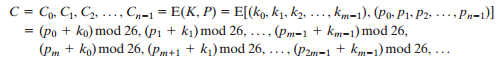
\includegraphics[scale=0.85]{images/bab2/poly.png}
		\begin{align*}
 		C &=c_0,c_1,c_2,...,c_{n-1} \\
      	E(K,P)&=E[(k_0,k_1,...,k_{m-1})(p_0,p_1,...,p_{n-1})] \\
      	&=(p_0+k_0)mod26,(p_1+k_1)mod26,...,(p_{m-1}+k_{m-1})mod26, \\
      		&(p_m+k_0)mod26,(p_{m+1}+k_1)mod26,...,(p_{2m-1}+k_{m-1})mod26,...
		\end{align*}		
		
		\caption{Aturan \textit{Polyalphabetical Cipher}}
		\label{fig:polyalphabeticalcipher}
	\end{figure}
	Di mana $C$ adalah \textit{ciphertext}, $E$ adalah fungsi enskripsi, $K$ adalah kunci, dan $P$ adalah \textit{plaintext}.
	Salah satu turunan dari \textit{polyalphabetic cipher} adalah teknik \textit{Vigenere Cipher} yang menjadi dasar permasalahan yang diangkat dalam tugas akhir ini\cite{stallings_computer_2015}.
	
	\subsection{Ciphertext}
	\textit{Ciphertext} adalah suatu pesan / teks acak yang dihasilkan dari suatu algoritma kriptografi. 
	Contoh dari \ciphertext dalam kasus \textit{polyalphabetical cipher} adalah "RTPPRKGFI" yang merupakan hasil enkripsi dari "PLAINTEXT" dan menggunakan kunci "CIPHER"\cite{william_crytography_2011}.
	
	\subsection{Plaintext}
	\textit{Plaintext} adalah data original sebagai inputan dari suatu metode enskripsi yang akan dilakukan\cite{william_crytography_2011}. Biasanya merupakan suatu rangkaian kata yang masih dapat dipahami artinya atau hasil keluaran dari suatu algoritma kriptografi yang akan dienskripsi lagi.
	
	\subsection{Secret Key}
	\textit{Secret Key} atau yang lebih dikenal dengan \textit{key} adalah suatu inputan dari algoritma enskripsi yang akan menentukan suatu transformasi dan subtitusi yang akan dilakukan oleh algoritma enskripsi\cite{william_crytography_2011}. Dalam kasus \textit{polyalphabetical cipher} pada permasalahan yang diangkat dalam tugas akhir ini, panjang kunci yang digunakan setidaknya 1. 
	
	\subsection{Friedman test}
	\textit{Friedman test} atau \textit{Kappa Test} merupakan salah satu metode yang digunakan untuk mendeskripsikan \textit{Polyalphabetical Cipher} dengan menggunakan \textit{index of coincidence}. \textit{Index of coincidence} digunakan untuk mengukur tingkat ketidakrataan frekuensi \textit{ciphertext}. Untuk menghitung \textit{index of coincidence} digunakan persamaan \ref{eq:12}\cite{henk_encyclopedia_2005}.
	\begin{equation} \label{eq:12}
	\begin{split}
	IC&=c*((\frac{n_a}{N}*\frac{n_a-1}{N-1})+(\frac{n_b}{N}*\frac{n_b-1}{N-1})+ \\
	&(\frac{n_c}{N}*\frac{n_c-1}{N-1})+...+(\frac{n_z}{N}*\frac{n_z-1}{N-1}))\\
	\end{split}
	\end{equation}
	Persamaan \ref{eq:12} dapat disederhanakan menjadi persamaan \ref{eq:13}.
	\begin{equation} \label{eq:13}
	IC=\frac{\sum_{i=1}^{c}n_i(n_i-1)}{\frac{N*(N-1)}{c}}
	\end{equation}
	$IC$ adalah \textit{index of coincidence}, $n_a$ adalah jumlah huruf "a" yang terdapat pada suatu \textit{ciphertext} dan seterusnya, $N$ adalah jumlah huruf yang terdapat pada \textit{ciphertext}, $c$ adalah jumlah huruf dalam alfabet. Karena tidak dapat mengetahui jumlah huruf yang mungkin terbentuk dalam alfabet yang ada dan harus mengetahui jumlah setiap huruf yang muncul dalam suatu \textit{ciphertext}. Karena keterbatasan informasi mengenai \ciphertext yang didapatkan, maka metode ini tidak dapat digunakan untuk menyelesaikan permasalahan dalam tugas akhir ini.
	
	 \subsection{Kasiski Examination}
	 \textit{Kasiski Examination} merupakan suatu teknik yang digunakan untuk mendeskripsikan secara paksa suatu \textit{ciphertext} yang menggunakan teknik substitusi, baik itu \textit{polyalphabetical cipher} maupun \textit{monoalphabetical cipher}. Teknik menggunakan kelemahan yang ditimbulkan oleh teknik substitusi itu sendiri. Yaitu apabila suatu \textit{subtring} dari \plaintext dan \textit{subtring} dari suatu set kunci yang berulang terdapat yang berulang, maka dapat dipastikan untuk menebak panjang huruf / karakter kunci yang digunakan, tanpa diketahui \plaintext dan kuncinya. Sebagai contoh dapat dilihat pada Tabel \ref{tab:kasiskiexamination}.
	 \begin{table}[H]
	 	\caption{Contoh \textit{Kasiski Examintaion}}
		\resizebox{\textwidth}{!}{%
		\begin{tabular}   {|c|c|c|c|c|c|c|c|c|c|c|c|c|c|c|c|}\hline
		\textit{ciphertext}&C&S&A&S&X&S&J&O&S&P&C&S&A&S&X \\ \hline
		%kunci              &a&b&c&d&e&a&b&c&d&e&a&b&c&d&e \\ \hline
		\end{tabular}}
		\label{tab:kasiskiexamination}
	\end{table}
	Dari Tabel \ref{tab:kasiskiexamination} yang ada dapat disimpulkan bahwa kata "CSASX" berulang. Sehingga setidaknya dapat disimpulkan bahwa panjang kuncinya mungkin 5 karakter atau faktor dari 10\cite{noauthor_kasiski_nodate}.
	Cara pencarian panjangnya:
	\begin{enumerate}
	\item Mencari semua subtring yang berulang. Seperti Tabel \ref{tab:kasiskiexamination}.
	\item Mencari semua faktor kapan subtring itu berulang lagi sebagai contoh Tabel \ref{tab:kasiskiexamination} itu selisih antara sub kalimat "CSASX" adalah 10. Maka, faktor dari 10 adalah 10,5,2,1. 
	\item Kemungkinan besar faktor yang sering berulang adalah jawabannya. 
	\end{enumerate}
	 Hal ini yang menjadi dasar pengerjaan permasalahan yang diangkat dalam tugas akhir ini.
 
	\subsection{Intersection}
	\textit{Intersection} adalah himpunan A dan himpunan B di mana ada bagian dari A juga merupakan bagian dari B. Sehingga dapat ditulis dengan persamaan \ref{eq:intersect}.
	\begin{equation}
	\label{eq:intersect}
	A\cap{B=\{x:x\in A \textrm{ dan } x \in B \}}
	\end{equation}
	Sebagai contoh \textit{intersection} antara $\{1,2,3\}$ dan $\{1,4,5\}$ adalah $\{1\}$\cite{devlin_joy_1993}	.
	
	\section{Deskripsi Permasalahan}
	\label{chapter:dasar-teori}
	Permasalahan yang diangkat dalam tugas akhir ini diangkat dari suatu permasalahan yang terdapat pada suatu situs penilaian daring atau \textit{online judge} SPOJ yaitu \textit{The Bytelandian Cryptographer (Act IV)} dengan nomer soal 20 dengan kode soal CRYPTO4. Deskripsi soal yang asli menggunakan bahasa Inggris dapat dilihat pada Gambar \ref{fig:crypto4_def}\cite{piwakowski_crypto4_2004}.
	
	
	 Permasalahan pada The Bytelandian Cryptographer (Act IV) diberikan pesan dengan panjang $N$ huruf, huruf yang digunakan adalah huruf kapital latin dari A sampai dengan Z, yang dapat ditafsirkan menjadi bilangan bulat dari 0 sampai dengan 25. Diberikan kunci untuk mentransmisikan pesan yang diketahui oleh kedua belah pihak yang terdiri dari $M$ bilangan bulat. Dengan menggunakan kunci yang ada bahwa pada index ke $i$ dari pesan pada index $x_i$ akan di enkripsikan ke dalam bentuk index ke $i$ dari pesan hasil enskripsi $y$, yang mengikuti aturan \ref{eq:hahah}.
	\begin{equation}
	y_i=x_i+k_{1+(i-1)mod M} mod 26 
	\label{eq:hahah}
	\end{equation}		 
	 Diketahui \textit{plaintext} dan \textit{ciphertext} yang diberikan hanya berupa potongan-potongan dari kedua pesan tersebut. Dicari bagaimana menkonstruksi ulang pesan yang telah didapat sehingga bisa membentuk \textit{plaintext} yang asli dari pesan yang telah didapatkan sebanyak-banyaknya.
	\begin{figure}[H]
		\centering
		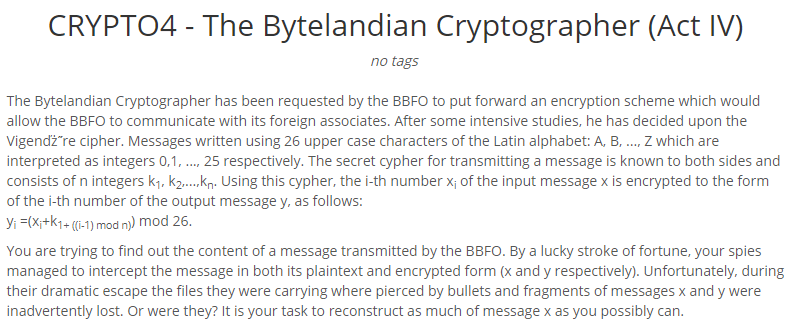
\includegraphics[scale=0.75]{images/bab2/crypto_def.png}
		\caption{Deskripsi Permasalahan dalam Bahasa Inggris pada SPOJ \textit{The Bytelandian Cryptographer (Act IV)}}
		\label{fig:crypto4_def}
	\end{figure}
	
	Deskripsi mengenai format masukan sebagai berikut:
	\begin{enumerate}
	\item Baris pertama berisi sejumalah $T$ kasus uji coba
	\item Setiap kasus uji coba, baris pertama berisi $1$ bilangan bulat $M$ dimana merupakan sejumlah batas atas panjang kunci yang digunakan 
	\item Baris kedua dari setiap kasus uji coba berisi \textit{plaintext}.
	\item Baris ketiga dari setiap kasus uji coba berisi \textit{ciphertext}.
	%\item \textit{Plaintext} dan \textit{ciphertext} direpresentasikan dengan karakter 'A' sampai dengan 'Z'.
	\end{enumerate}
	\textit{Plain text} dan \textit{ciphertext} dalam format masukan menggunakan karakter A sampai dengan Z yang dapat ditafsirkan kedalam bilangan bulat 0 sampai dengan 25 dan karakter '*' yang dapat ditafsirkan sebagai karakter yang hilang.
	
	
	Format keluaran yang dihasilkan adalah 1 baris \textit{plaintext} yang dapat direkontruksi dan '*' apabila nilai dari karakter pada posisi tersebut tidak dapat ditentukan. 
	Batasan permasalahan \textit{The Bytelandian Cryptographer (Act IV)} adalah sebagai berikut:
	\begin{enumerate}
		\item $T \leq 200$
		\item $1 \leq M \leq 100,000$
		\item Panjang \textit{input file} tidak melebihi dari 2MB.
		\item Lingkungan penilaian Intel Pentium G860 3GHz.
		\item Batas Waktu: $\leq17$ detik
		\item Batas Sumber Code : 50000B
		\item Batas Memory : 1536 MB.                 
	\end{enumerate}

	\section{Contoh Kasus Permasalahan}
	Dalam Permasalahan yang diangkat ini huruf A sampai dengan Z ditafsirkan sebagai 0 sampai dengan 25.
	Contoh 1. Diketahui $M$ bernilai 1 yang menunjukkan batas atas dari panjang kunci. Diketahui \plaintext adalah A*X*C dan \ciphertext adalah **CM*. 
	\begin{table}[H]
	 	\centering
		\caption{Contoh 1}	 	
	 	\begin{tabular}{|c|c|c|c|c|c|c|}\hline
	 	\textit{index}&0&1&2&3&4\\ \hline
	 	\textit{plain text}&A&*&X&*&C\\ \hline
	 	\textit{ciphertext}&*&*&C&M&*\\ \hline
	 	Selisih yang diketahui& & &5& & \\ \hline
	 	Hasil              &A&*&X&H&C\\ \hline
	 	\end{tabular}
	 	\label{tab:contoh1}
	\end{table}
	 
	 Dari Tabel \ref{tab:contoh1} dapat diketahui bagaimana hasil yang akan dicapai. Cara mencapai hasil yang diinginkan adalah sebagai berikut. Pertama-tama pencarian panjang kunci. Pada pencarian panjang kunci harus mengetahui dahulu batas atas dari panjang kunci tersebut. Pada contoh kasus ini $M$ bernilai 1, maka kemungkinan jawabannya hanya ada 1, yaitu $M$ itu sendiri, karena suatu panjang kunci yang digunakan dalam enskripsi tidak mungkin 0. Diasumsikan bahwa 1 warna mewakili satu blok kunci yang akan digunakan. Maka akan membentuk seperti pada Tabel \ref{tab:langkah1contoh1}.
	 
	\begin{table}[H]
	 	\centering
		\caption{Langkah 1 Contoh 1}	 	
	 	\setlength{\arrayrulewidth}{.08em}
	 	\begin{tabular}{|c|c|c|c|c|c|c|}\hline
	 	\textit{index}&0&1&2&3&4\\ \hline
	 	\textit{plain text}&\cellcolor{blue!15}A&\cellcolor{lime!15}*&\cellcolor{yellow!25}X&\cellcolor{green!15}*&\cellcolor{pink!25}C\\ \hline
	 	\textit{ciphertext}&\cellcolor{blue!15}*&\cellcolor{lime!15}*&\cellcolor{yellow!25}C&\cellcolor{green!15}M&\cellcolor{pink!25}*\\ \hline
	 	Selisih yang diketahui& & &5& & \\ \hline
	 	%Hasil              &A&*&X&H&C\\ \hline
	 	\end{tabular}
	 	\label{tab:langkah1contoh1}
	\end{table}
	
	  Karena selisih yang di ketahui hanya ada 1, maka itulah yang menjadi jawabannya. Selanjutnya mencari yang \plaintext yang bernilai "*" dan \ciphertext tidak kosong, seperti indeks ketiga. Maka indeks ketiga jawabannya adalah "H". Karena "M" $-$ $5$ adalah "H".
	 
	 
	 
	 Contoh 2. Diketahui bahwa $M$ bernilai 4 yang menunjukkan batas atas dari panjang kunci. Diketahui \plaintext adalah *B***A dan \ciphertext adalah AAAAAA. Dalam Contoh ini panjang kuncinya bisa dari 1 sampai dengan 4. 
	 \begin{table}[H]
	 	\centering
	 	\caption{Contoh 2}
	 	\begin{tabular}{|c|c|c|c|c|c|c|}\hline
		\textit{index}&0&1&2&3&4&5\\ \hline
	 	\textit{plain text}&*&B&*&*&*&A\\ \hline
	 	\textit{ciphertext}&A&A&A&A&A&A\\ \hline
	 	Selisih yang diketahui& &25& & & &0\\ \hline
	 	Panjang Kunci 1 & \multicolumn{6}{c|}{tidak bisa karena ada yang \textit{collision}}\\ \hline
	 	Panjang Kunci 2 & \multicolumn{6}{c|}{tidak bisa karena ada yang \textit{collision}}\\ \hline
	 	Panjang Kunci 3 &*&B&A&*&B&A \\ \hline
	 	Panjang Kunci 4 & \multicolumn{6}{c|}{tidak bisa karena ada yang \textit{collision}}\\ \hline
	 	\end{tabular}
	 	\label{tab:contoh2}
	\end{table}
	Cara yang harus dilalui adalah sebagai berikut. Pertama mencari panjang kunci yang bernilai diantara 1 - 4. \\
	Pada Tabel \ref{tab:k1contoh2} akan diperlihatkan proses pencarian ketika panjang kunci adalah 1.
	\begin{table}[H]
	 	\centering
	 	\caption{Panjang Kunci 1 Contoh 2}
	 	\setlength{\arrayrulewidth}{.08em}
	 	\begin{tabular}{|c|c|c|c|c|c|c|}\hline
		\textit{index}&0&1&2&3&4&5\\ \hline
	 	\textit{plain text}&\cellcolor{blue!15}*&\cellcolor{yellow!25}B&\cellcolor{green!15}*&\cellcolor{lime!25}*&\cellcolor{pink!30}*&\cellcolor{red!25}A\\ \hline
	 	\textit{ciphertext}&\cellcolor{blue!15}A&\cellcolor{yellow!25}A&\cellcolor{green!15}A&\cellcolor{lime!25}A&\cellcolor{pink!30}A&\cellcolor{red!25}A\\ \hline
	 	Selisih yang diketahui& &25& & & &0\\ \hline
	 	Panjang Kunci 1 & \multicolumn{6}{c|}{tidak bisa karena ada yang \textit{collision}}\\ \hline
	 	\end{tabular}
	 	\label{tab:k1contoh2}
	\end{table}	
	
	Apabila $1$ warna direpresentasikan menjadi 1 blok kunci, maka terdapat 5 blok kunci yang terbentuk. Pada bagian Tabel \ref{tab:k1contoh2} bahwa hanya ada 2 indeks di mana \plaintext dan \ciphertext yang diketahui. Kedua-duanya terletak pada blok kunci yang berbeda. Akan tetapi karena panjang bloknya $1$ maka tidak mungkin panjang kunci 1 dilakukan karena kedua-duanya saling bertabrakan dan membawa nilai yang berbeda. Yang menjadi permasalahan pada panjang kunci 1 adalah ketika blok yang diketahui bertabrakan dan masing masing membawa nilai yang berbeda juga. Sehinnga dapat disimpulkan bahwa panjang kunci 1 pada contoh kasus 2 tidak mungkin terjadi.
	\\
	Proses pencarian ketika panjang kunci adalah 2.
	\begin{table}[H]
	 	\centering
	 	\caption{Panjang Kunci 2 Contoh 2}
	 	\setlength{\arrayrulewidth}{.08em}
	 	\begin{tabular}{|c|c|c|c|c|c|c|}\hline
		\textit{index}&0&1&2&3&4&5\\ \hline
	 	\textit{plain text}&\cellcolor{blue!15}*&\cellcolor{blue!15}B&\cellcolor{green!15}*&\cellcolor{green!15}*&\cellcolor{pink!30}*&\cellcolor{pink!30}A\\ \hline
	 	\textit{ciphertext}&\cellcolor{blue!15}A&\cellcolor{blue!15}A&\cellcolor{green!15}A&\cellcolor{green!15}A&\cellcolor{pink!30}A&\cellcolor{pink!30}A\\ \hline
	 	Selisih yang diketahui& &25& & & &0\\ \hline
	 	Panjang Kunci 2 & \multicolumn{6}{c|}{tidak bisa karena ada yang \textit{collision}}\\ \hline
	 	\end{tabular}
	 	\label{tab:k2contoh2}
	\end{table}	
	
	Apabila 1 warna direprentasikan menjadi 1 blok kunci, maka terdapat 3 blok kunci yang terbentuk. Pada Tabel \ref{tab:k2contoh2} terlihat bahwa terdapat 2 indeks di mana \plaintext dan \ciphertext yang diketahui. Indeks yang pertama terletak pada blok pertama bagian akhir, begitu juga indeks yang kedua terletak pada blok 3 bagian akhir. Karena kedua-duanya terletak pada bagian akhir dari masing-masing blok maka dapat disimpulkan panjang kunci 2 juga tidak dapat digunakan.
	\\
	Proses Pencarian ketika panjang kunci adalah 3.
	\begin{table}[H]
	 	\centering
	 	\caption{Panjang Kunci 3 Contoh 2}
	 	\setlength{\arrayrulewidth}{.08em}
	 	\begin{tabular}{|c|c|c|c|c|c|c|}\hline
		\textit{index}&0&1&2&3&4&5\\ \hline
	 	\textit{plain text}&\cellcolor{blue!15}*&\cellcolor{blue!15}B&\cellcolor{blue!15}*&\cellcolor{green!15}*&\cellcolor{green!15}*&\cellcolor{green!15}A\\ \hline
	 	\textit{ciphertext}&\cellcolor{blue!15}A&\cellcolor{blue!15}A&\cellcolor{blue!15}A&\cellcolor{green!15}A&\cellcolor{green!15}A&\cellcolor{green!15}A\\ \hline
	 	Selisih yang diketahui& &25& & & &0\\ \hline
	 	Panjang Kunci 3 &*&B&A&*&B&A \\ \hline
	 	\end{tabular}
	 	\label{tab:k3contoh2}
	\end{table}	
	Apabila 1 warna direpresentasikan menjadi 1 blok kunci, maka terdapat 2 blok kunci yang terbentuk. Pada Tabel \ref{tab:k3contoh2} terlihat bahwa terdapat 2 indeks di mana \plaintext dan \ciphertext yang diketahui. Indeks yang pertama terletak dibagian tengah pada blok 1 dan indeks yang kedua terletak pada bagian akhir pada blok 2. Maka,  \plaintext yang terbentuk adalah pada bagian akhir dari blok kunci 1 dan bagian tengah dari blok kunci 2. Karena kedua-duanya saling melengkapi antara satu bagian dengan bagian lainnya. Sehingga hasil yang terbentuk pada bagian akhir dari blok kunci 1 adalah "A" $-$ $0$ adalah "A" dan bagian tengah dari blok kunci 2 adalah "A" $-$ $25$ adalah "B". 
	\\
	Proses pencarian ketika panjang kunci adalah 4
	\begin{table}[H]
	 	\centering
	 	\caption{Panjang Kunci 4 Contoh 2}
	 	\setlength{\arrayrulewidth}{.08em}
	 	\begin{tabular}{|c|c|c|c|c|c|c|}\hline
		\textit{index}&0&1&2&3&4&5\\ \hline
	 	\textit{plain text}&\cellcolor{blue!15}*&\cellcolor{blue!15}B&\cellcolor{blue!15}*&\cellcolor{blue!15}*&\cellcolor{green!15}*&\cellcolor{green!15}A\\ \hline
	 	\textit{ciphertext}&\cellcolor{blue!15}A&\cellcolor{blue!15}A&\cellcolor{blue!15}A&\cellcolor{blue!15}A&\cellcolor{green!15}A&\cellcolor{green!15}A\\ \hline
	 	Selisih yang diketahui& &25& & & &0\\ \hline
	 	Panjang Kunci 4 & \multicolumn{6}{c|}{tidak bisa karena ada yang \textit{collision}}\\ \hline
	 	\end{tabular}
	 	\label{tab:k4contoh2}
	\end{table}	
	Apabila 1 warna direpresentasikan menjadi 1 blok kunci, maka terdapat 2 blok kunci yang terbentuk. Pada Tabel \ref{tab:k4contoh2} terlihat bahwa terdapat 2 indeks di mana \plaintext dan \ciphertext yang diketahui. Indeks yang pertama terletak dibagian kedua dari depan pada blok 1 dan indeks yang kedua terletak pada bagian kedua dari depan pada blok 2. Maka dalam ini tidak bisa digunakan panjang kunci 4, karena terdapat bagian dari kedua blok pada panjang kunci 4 yang bertabrakan dan membawa nilai yang berbeda. Sehingga hasil yang terbentuk dapat dilihat pada Tabel \ref{tab:rescontoh2}
	
	\begin{table}[H]
	 	\centering
	 	\caption{Hasil Contoh 2}
	 	\setlength{\arrayrulewidth}{.08em}
	 	\begin{tabular}{|c|c|c|c|c|c|c|}\hline
		\textit{index}&0&1&2&3&4&5\\ \hline
	 	\textit{plain text}&*&B&*&*&*&A\\ \hline
	 	\textit{ciphertext}&A&A&A&A&A&A\\ \hline
	 	Selisih yang diketahui& &25& & & &0\\ \hline
	 	Hasil &*&B&A&*&B&A \\ \hline
	 	\end{tabular}
	 	\label{tab:rescontoh2}
	\end{table}	 
	
		
	Contoh 3. Diketahui bahwa $M$ bernilai 4 yang menunjukkan batas atas dari panjang kunci. Diketahui \plaintext adalah *AA******* dan \ciphertext adalah AAAAAAAAAA. Indeks akan dihitung mulai dari 0. 
	 \begin{table}[H]
	 	\centering
	 	\caption{Contoh 3}
	 	\begin{tabular}{|c|c|c|c|c|c|c|c|c|c|c|}\hline
	 	\textit{index}&0&1&2&3&4&5&6&7&8&9\\ \hline
	 	\textit{plain text}&*&A&A&*&*&*&*&*&*&*\\ \hline
	 	\textit{ciphertext}&A&A&A&A&A&A&A&A&A&A\\ \hline
		Selisih yang diketahui & &0&0& & & & & & & \\ \hline	 	
	 	\end{tabular}
	 	\label{tab:contoh3}
	\end{table}
	
	Cara yang harus dilalui adalah sebagai berikut. Pertama mencari panjang kunci yang bernilai diantara 1 - 4. \\
	Pada Tabel \ref{tab:k1contoh3} akan diperlihatkan proses pencarian ketika panjang kunci adalah 1.
	\begin{table}[H]
	 	\centering
	 	\caption{Panjang Kunci 1 Contoh 3}
	 	\setlength{\arrayrulewidth}{.08em}
	 	\begin{tabular}{|c|c|c|c|c|c|c|c|c|c|c|}\hline
	 	\textit{index}&0&1&2&3&4&5&6&7&8&9\\ \hline
	 	\textit{plain text}&\cellcolor{blue!15}*&\cellcolor{yellow!25}A&\cellcolor{green!15}A&\cellcolor{lime!25}*&\cellcolor{pink!30}*&\cellcolor{red!15}*&\cellcolor{violet!30}*&\cellcolor{magenta!15}*&\cellcolor{purple!25}*&\cellcolor{teal!35}*\\ \hline
	 	\textit{ciphertext}&\cellcolor{blue!15}A&\cellcolor{yellow!25}A&\cellcolor{green!15}A&\cellcolor{lime!25}A&\cellcolor{pink!30}A&\cellcolor{red!15}A&\cellcolor{violet!30}A&\cellcolor{magenta!15}A&\cellcolor{purple!25}A&\cellcolor{teal!35}A\\ \hline
		Selisih yang diketahui & &0&0& & & & & & & \\ \hline	
		Panjang kunci 1 &A&A&A&A&A&A&A&A&A&A\\ \hline 	
	 	\end{tabular}
	 	\label{tab:k1contoh3}
	\end{table}
	
	Apabila 1 warna merepresentasikan sebagai 1 blok kunci maka, dapat terbentuk sebanyak 10 blok kunci. Dapat dilihat pada Tabel \ref{tab:k1contoh3}. Indeks yang diketahui baik \plaintext dan \ciphertext adalah indeks 1 dan indeks 2, yang mana keduanya terletak pada blok yang berbeda. Akan tetapi, karena mereka membawa 1 nilai yang sama maka semua plaintext yang kosong pasti bernilai "A".
	\\
	Pada Tabel \ref{tab:k2contoh3} akan diperlihatkan proses pencarian ketika panjang kunci adalah 2.
	\begin{table}[H]
	 	\centering
	 	\caption{Panjang Kunci 2 Contoh 3}
	 	\setlength{\arrayrulewidth}{.08em}
	 	\begin{tabular}{|c|c|c|c|c|c|c|c|c|c|c|}\hline
	 	\textit{index}&0&1&2&3&4&5&6&7&8&9\\ \hline
	 	\textit{plain text}&\cellcolor{blue!15}*&\cellcolor{blue!15}A&\cellcolor{green!15}A&\cellcolor{green!15}*&\cellcolor{pink!30}*&\cellcolor{pink!30}*&\cellcolor{violet!30}*&\cellcolor{violet!30}*&\cellcolor{purple!25}*&\cellcolor{purple!25}*\\ \hline
	 	\textit{ciphertext}&\cellcolor{blue!15}A&\cellcolor{blue!15}A&\cellcolor{green!15}A&\cellcolor{green!15}A&\cellcolor{pink!30}A&\cellcolor{pink!30}A&\cellcolor{violet!30}A&\cellcolor{violet!30}A&\cellcolor{purple!25}A&\cellcolor{purple!25}A\\ \hline
		Selisih yang diketahui & &0&0& & & & & & & \\ \hline	
		Panjang kunci 2 &A&A&A&A&A&A&A&A&A&A\\ \hline 	
	 	\end{tabular}
	 	\label{tab:k2contoh3}
	\end{table}
	Apabila 1 warna merepresentasikan sebagai 1 blok kunci maka, dapat terbentuk sebanyak 5 blok kunci. Dapat dilihat pada Tabel \ref{tab:k2contoh3}. Indeks yang diketahui baik \plaintext dan \ciphertext adalah indeks 1 dan indeks 2, yang mana keduanya terletak pada blok yang berbeda dan posisi yang berbeda pula. Hal ini dapat dilihat pada Tabel \ref{tab:k2contoh3}. Indeks yang diketahui pertama terletak pada bagian akhir dari blok 1 dan indeks yang diketahui kedua terletak pada bagian awal dari blok 2. Maka dapat disimpulkan bahwa seluruh plaintext yang nilai "*" dan ciphertext yang nilainya tidak "*", nilai dari plaintext yang terbentuk seluruhnya "A", seperti yang terlihat pada Tabel \ref{tab:k2contoh3}.
	\\	
	Pada Tabel \ref{tab:k3contoh3} akan diperlihatkan proses pencarian ketika panjang kunci adalah 3.
	\begin{table}[H]
	 	\centering
	 	\caption{Panjang Kunci 3 Contoh 3}
	 	\setlength{\arrayrulewidth}{.08em}
	 	\begin{tabular}{|c|c|c|c|c|c|c|c|c|c|c|}\hline
	 	\textit{index}&0&1&2&3&4&5&6&7&8&9\\ \hline
	 	\textit{plain text}&\cellcolor{blue!15}*&\cellcolor{blue!15}A&\cellcolor{blue!15}A&\cellcolor{blue!15}*&\cellcolor{green!15}*&\cellcolor{green!15}*&\cellcolor{green!15}*&\cellcolor{green!15}*&\cellcolor{violet!30}*&\cellcolor{violet!30}*\\ \hline
	 	\textit{ciphertext}&\cellcolor{blue!15}A&\cellcolor{blue!15}A&\cellcolor{blue!15}A&\cellcolor{blue!15}A&\cellcolor{green!15}A&\cellcolor{green!15}A&\cellcolor{green!15}A&\cellcolor{green!15}A&\cellcolor{violet!30}A&\cellcolor{violet!30}A\\ \hline
		Selisih yang diketahui & &0&0& & & & & & & \\ \hline	
		Panjang kunci 3 &*&A&A&*&A&A&*&A&A&*\\ \hline 	
	 	\end{tabular}
	 	\label{tab:k3contoh3}
	\end{table}
	Apabila 1 warna merepresentasikan sebagai 1 blok kunci maka, dapat terbentuk sebanyak 4 blok kunci. Dapat dilihat pada Tabel \ref{tab:k3contoh3}. Indeks yang diketahui baik \plaintext dan \ciphertext adalah indeks 1 dan indeks 2, di mana smuanya terletak pada satu blok yang sama, yaitu blok kunci 1 . Jadi, sisanya menngikuti perulangan dari blok kunci 1. 
	\\
	Pada Tabel \ref{tab:k4contoh3} akan diperlihatkan proses pencarian ketika panjang kunci adalah 4.
	\begin{table}[H]
	 	\centering
	 	\caption{Panjang Kunci 4 Contoh 3}
	 	\setlength{\arrayrulewidth}{.08em}
	 	\begin{tabular}{|c|c|c|c|c|c|c|c|c|c|c|}\hline
	 	\textit{index}&0&1&2&3&4&5&6&7&8&9\\ \hline
	 	\textit{plain text}&\cellcolor{blue!15}*&\cellcolor{blue!15}A&\cellcolor{blue!15}A&\cellcolor{green!15}*&\cellcolor{green!15}*&\cellcolor{green!15}*&\cellcolor{violet!30}*&\cellcolor{violet!30}*&\cellcolor{violet!30}*&\cellcolor{purple!25}*\\ \hline
	 	\textit{ciphertext}&\cellcolor{blue!15}A&\cellcolor{blue!15}A&\cellcolor{blue!15}A&\cellcolor{green!15}A&\cellcolor{green!15}A&\cellcolor{green!15}A&\cellcolor{violet!30}A&\cellcolor{violet!30}A&\cellcolor{violet!30}A&\cellcolor{purple!25}A\\ \hline
		Selisih yang diketahui & &0&0& & & & & & & \\ \hline	
		Panjang kunci 4 &*&A&A&*&*&A&A&*&*&A\\ \hline 	
	 	\end{tabular}
	 	\label{tab:k4contoh3}
	\end{table}
	Apabila 1 warna merepresentasikan sebagai 1 blok kunci maka, dapat terbentuk sebanyak 4 blok kunci. Dapat dilihat pada Tabel \ref{tab:k4contoh3}. Indeks yang diketahui baik \plaintext dan \ciphertext adalah indeks 1 dan indeks 2, di mana smuanya terletak pada satu blok yang sama, yaitu blok kunci 1 . Jadi, sisanya menngikuti perulangan dari blok kunci 1. 
	
	\begin{table}[H]
		\centering
		\caption{Hasil dari Contoh 3}
		\begin{tabular}{|c|c|c|c|c|c|c|c|c|c|c|}\hline
		\textit{index}&0&1&2&3&4&5&6&7&8&9\\ \hline	
		\textit{plain text} awal&*&A&A&*&*&*&*&*&*&*\\ \hline
		Panjang kunci 1 &A&A&A&A&A&A&A&A&A&A\\ \hline
		Panjang kunci 2 &A&A&A&A&A&A&A&A&A&A\\ \hline
		Panjang kunci 3 &*&A&A&*&A&A&*&A&A&*\\ \hline
		Panjang kunci 4 &*&A&A&*&*&A&A&*&*&A\\ \hline
		Hasil Akhir     &*&A&A&*&*&A&*&*&*&*\\ \hline
		\end{tabular}
		\label{tab:res_contoh_3}
	\end{table}
	Pada Contoh ini kalau dilihat pada indeks selisih yang telah diketahui, terjadi bahwa panjang kunci 1 sampai dengan 4 dapat tercipta sedangkan pada contoh sebelumnya tidak bisa. Hal ini juga di pengaruhi oleh karena isinya itu sama. Walaupun terjadi \textit{collision} pada indeks yang selisih yang diketahui, tetapi kalau hasilnya sama maka hal itu jawaban untuk setiap panjang kunci bisa terbentuk. Keempat panjang kunci tersebut benar terhadap pesan tersebut. Hasil keluaran yang diinginkan hanya 1 saja tetapi keempat-empatnya benar, oleh karena itu perlu dilakukan \textit{intersection} atau perpotongan dari himpunan keempat kunci tersebut. Perpotongan itu menghasilkan {,A,A,,A,,,,,}. Terdapat bagian bagian yang kosong yang dapat  diisi dengan *. Sehingga hasil akhirnya dapat dilihat pada Tabel \ref{tab:res_contoh_3} pada bagian hasil akhir.
	
	\section{Penyelesaian Masalah The Bytelandian Cryptographer (Act IV)}
	\label{chapter:solving}
	Permasalahan \textit{The Bytelandian Cryptographer (Act IV)} dapat diselesaikan dengan menggunakan \textit{Kasiski Examination} dan \textit{Intersection}. Untuk menyelesaikan masalah ini perlu ditafsirkan bahwa karakter A sampai dengan Z menjadi 0 sampai dengan 25, karena untuk memudahkan perhitungan mencari selisih dan merekonstruksi \plaintext dari \ciphertext dan karakter kunci. Berikut ini tahapan-tahapan untuk menyeselsaikan masalah ini:
	\begin{enumerate}
	\item Menyimpan posisi indeks karakter, di mana pada indeks tersebut baik \ciphertext maupun \plaintext tidak bernilai '*', beserta menyimpan hasil perhitungan selisih antara \ciphertext dan \plaintext\cite{john_jones_spoj_2009}.
	\item Menyimpan posisi indeks, apabila  \ciphertext diketahui dan \plaintext tidak diketahui. Untuk mengurangi \textit{running time} dari program\cite{john_jones_spoj_2009}.
	\item Pada Tahapan ini adalah modifikasi dari \textit{Kasiski Examnination}, apabila menggunakan \textit{Kasiski Examination} pada umumnya yang hanya mencari posisi berulang dari suatu sub kalimat dalam suatu kalimat tidak bisa digunakan untuk menyelesaikan permaslahan ini. Oleh karena itu dirubah menjadi mengiterasi $M$ dari 1 sampai dengan $M$, yang akan digunakan untuk membagi selisih yang diketahui antara \plaintext dan \ciphertext sebesar posisi iterasi yang telah berjalan. Melihat apakah dalam blok-blok yang telah terbentuk ini terdapat \textit{collision} dan indeks yang saling bertabrakan memiliki nilai yang sama atau tidak, apabila sama maka tidak terjadi tabrakan sebalik jika terjadi tabrakan maka harus mencari panjang kunci yang baru. Mengiterasi panjang kunci dari $\frac{M}{2}+1<=N<=M$, alasannya dimulai dari $\frac{M}{2}+1$ tidak dari $1$ karena apabila suatu panjang kunci bernilai benar maka kelipatan dari panjang kunci itu pun juga pasti benar dan untuk mempersingkat waktu \textit{running time} yang seharusnya terjadi. Yang mendasari ini adalah dari Tabel  \ref{tab:contoh2} pada bagian 2.2. Pada bagian ini dilakukan untuk mencari panjang kunci yang benar dengan cara mengiterasi hasil yang diperoleh pada tahap 1 dimodulo dengan posisi iterasi yang dilakukan, apabila tidak terjadi konflik maka panjang kunci tersebut benar jika sebaliknya yang terjadi maka panjang kunci tersebut tidak salah. Contohnya dapat dilihat pada contoh 2 pada bagian 2.2. Pada bagian ini memungkinkan bahwa bisa jadi lebih dari 1 panjang kunci yang bernilai benar. Contohnya seperti yang terjadi pada Tabel \ref{tab:contoh3} pada bagian 2.2. 
	\item Melakukan \textit{intersection} terhadap himpunan dari kunci yang telah di hasilkan\cite{john_jones_spoj_2009}. \textit{intersection} yang dilakukan berada didalam perulangan panjang kunci pada waktu generate setiap karakter yang terdapat dalam penyimpanan tahap 2 pada panjang kunci tersebut dengan ketentuan:
	\begin{enumerate}
	\item Panjang kunci yang terbentuk harus benar.
	\item Apabila terdapat indeks yang tidak dapat dipastikan isinya maka posisinya harus di buang dari penyimpanan dan hasil yang diperoleh pasti '*'.
	\item Apabila \plaintext pada indeks tersebut nilainya masih '*' dan pada penyimpanan masih menyimpan indeks tersebut maka, hasilnya adalah \ciphertext pada indeks tersebut dikurangi dengan hasil yang diperoleh dari tahap 1 bagian perhitungan selisih pada indeks yang sama kemudian dimodulo 26.
	\end{enumerate}
	\end{enumerate}
	Sehingga untuk setiap \textit{textcase} kompleksitasnya 
	$$\mathcal{O}(T*\frac{M}{2}*(N+S))$$ 
	Di mana $\frac{M}{2}$ adalah batas atas kunci dibagi dengan $2$, $N$ adalah jumlah posisi karakter yang terdapat pada tahap 2, dan $S$ adalah jumlah posisi karakter yang terdapat pada tahap 1. Pada kondisi \textit{worst case} $T*(N+S)=1.000.000$, sedangkan $\frac{M}{2}$ adalah $50.000$. Hasilnya $50$ miliar perulangan, dengan asumsi $1$ detik adalah $1$ miliar perulangan maka waktu yang dibutuhkan adalah $50$ detik. Oleh karena itu hal ini tidak mungkin bisa dilakukan begitu saja, diperlukan pruning pada sumber kode yang ada untuk memangkas waktu eksekusi program.
    %\usepackage[noend]{algpseudocode}
\chapter{DESAIN}
\label{chapter:design}
Pada bab ini akan dijelaskan mengenai desain algoritma yang digunakan untuk menyelesaikan permasalahan pada Tugas Akhir ini.
\section{Desain Umum Sistem}	
Sistem pertama kali akan menjalankan fungsi MAIN terlebih dahulu. Desain dari fungsi main sendiri dapat dilihat pada gambar \ref{fig:mainfx}. Didalam fungsi main akan di panggil fungsi SOLVE yang digunakan untuk menyelesaikan permasalahan yang diangkat pada tugas akhir ini dan didalam fungsi SOLVE akan terdapat fungsi VALIDITY yang digunakan untuk mengecek kebenaran suatu panjang kunci yang sedang diproses. Secara garis besar fungsi Main.


\begin{figure}[H]
		\centering
		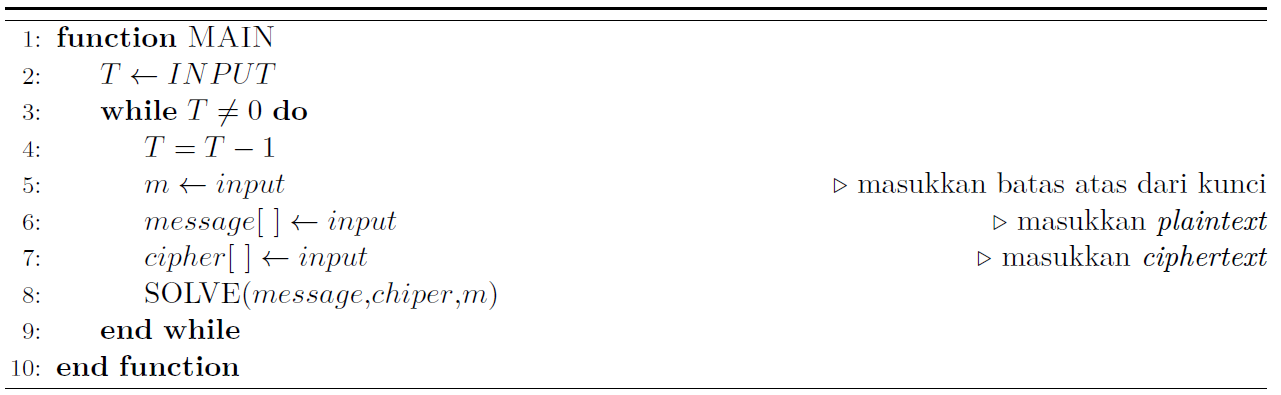
\includegraphics[scale=0.5]{images/bab3/mainfx.png}
		\caption{Gamba Fungsi Main}
		\label{fig:mainfx}
	\end{figure}

\section{Desain Algoritma}
 Pada bagian ini akan dibahas secara rinci mengenai fungsi-fungsi yang digunakan dalam sistem.  
  \subsection{Desain fungsi SOLVE}
  \label{chapter:fxsolve}
  Fungsi ini digunakan untuk menyelesaikan permasalahan yang diangkat pada tugas akhir ini yang didalamnya terdapat tahapan yang telah disebutkan di subbab \ref{chapter:dasar-teori} dan subbab \ref{chapter:solving}, kecuali untuk mengecek kebenaran dari suatu panjang kunci. Gambar mengenai fungsi SOLVE dapat dilihat pada gambar \ref{fig:solvefx}. Mengenai modulo 26 yang terdapat pada gambar digunakan untuk memastikan bahwa sesilih dari \plaintext dan \ciphertext adalah 0 sampai dengan 25, dan ditambah 26 pada gambar dimaksudkan agar silisih antara \plaintext dan \ciphertext selalu bernilai positif.
  
  \begin{figure}[H]
		\centering
		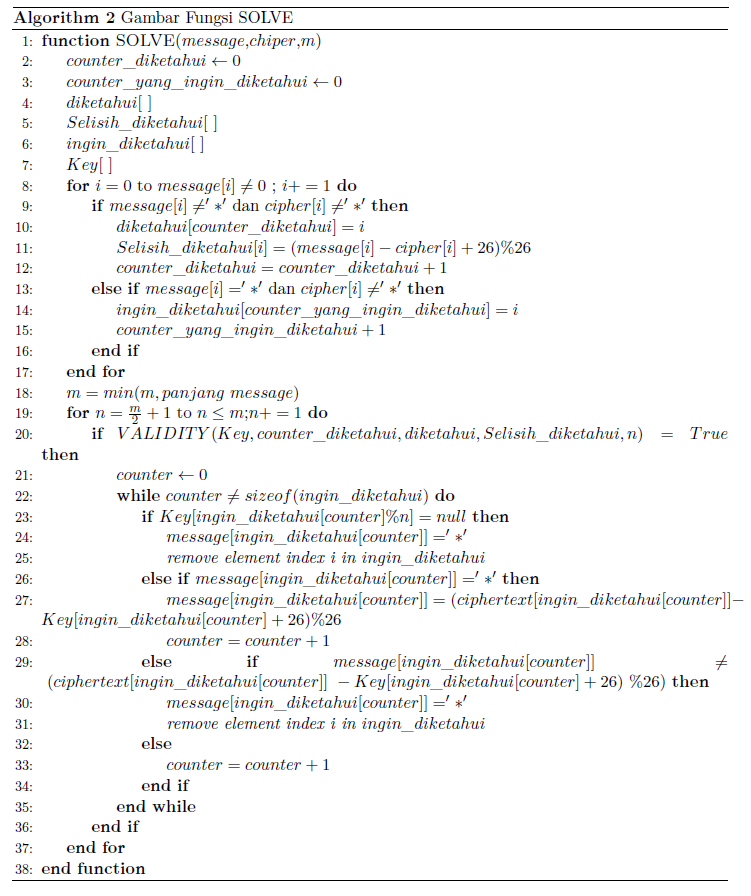
\includegraphics[scale=0.62]{images/bab3/solvefx.png}
		\caption{Gambar Fungsi SOLVE}
		\label{fig:solvefx}
	\end{figure}
	
	\subsection{Desain Fungsi VALIDITY}
	Fungsi ini digunakan untuk memvalidasi suatu panjang kunci yang sekarang di cek kebenarannya. Gambar mengenai fungsi VALIDITY dapat dilihar pada gambar \ref{fig:validity}. Penjelasan mengenai fungsi ini terdapat pada subbab \ref{chapter:solving}
	
 \begin{figure}[H]
		\centering
		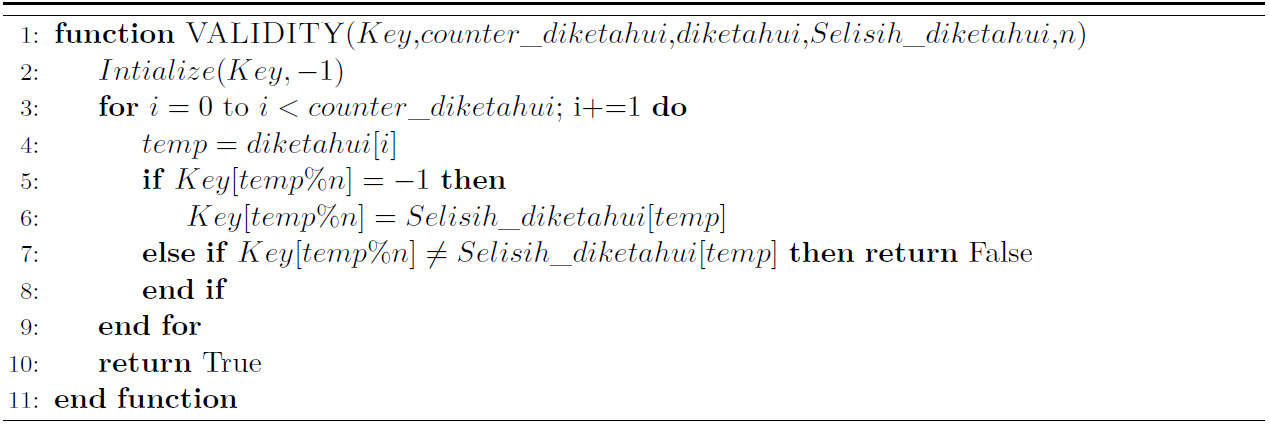
\includegraphics[scale=0.5]{images/bab3/validity.png}
		\caption{Gambar Fungsi VALIDITY}
		\label{fig:validity}
	\end{figure}
    \renewcommand\thelstlisting{\arabic{chapter}.\arabic{lstlisting}}
\chapter{IMPLEMENTASI}
  Pada bab ini menjelaskan implementasi yang sesuai dengan desain algoritma yang telah ditentukan sebelumnya.
  
  \section{Lingkungan Implementasi}
  Lingkungan uji coba yang digunakan adalah sebagai berikut:
  \begin{enumerate}
  \item Perangkat Keras
  	\begin{itemize}
  		\item \textit{Processor} Intel(R) Core(TM)i7-5700 @ 2.7GHz.
  		\item Memori 8 GB
  	\end{itemize}
  	\item Perangkat Lunak
  		\begin{itemize}
  		\item Sistem Operasi Windows 10 Home 64 bit
  		\item \textit{Text editor} Bloodshed Dev-C++ 5.11.
		\item \textit{Compiler} g++ (TDM-GCC 4.9.2 32-bit).
  		\end{itemize}
  \end{enumerate}
  \section{Rancangan Data}
Pada subbab ini dijelaskan mengenai desain data masukan yang
diperlukan untuk melakukan proses algoritma, dan data keluaran
yang dihasilkan oleh program.

\subsection{Data Masukan}
Data masukan adalah data yang akan diproses oleh program sebagai masukan menggunakan algoritma yang telah dirancang dalam tugas akhir ini.

Data masukan berupa berkas teks yang berisi data dengan format yang telah ditentukan pada deskripsi \textit{The Bytelandian Cryptographer (Act IV)}. Pada masing-masing berkas data masukan, baris pertama berupa sebuah bilangan bulat yang merepresentasikan jumlah kasus uji yang ada pada berkas tersebut. Untuk setiap kasus uji, baris pertama berupa sebuah bilangan bulat yang merepresentasikan batas atas dari kunci. baris kedua berupa \textit{string} yang merepresentasikan \plaintext dan baris ketiga berupa \textit{string} yang merepresentasikan \ciphertext.


\subsection{Data Keluaran}
Data keluaran yang dihasilkan oleh program hanya berupa satu kalimat yang berisikan \plaintext yang bisa didapatkan dari \ciphertext dan batas atas panjang kunci yang telah di berikan.

\section{Implementasi Algoritma dan Struktur Data}
Pada subbab ini akan dijelaskan tentang implementasi proses
algoritma secara keseluruhan berdasarkan desain yang telah
dijelaskan pada bab \ref{chapter:design}. Pada bagian ini menggunakan kode untuk mengoptimasi kompiler yang bertujuan untuk mempersingkat waktu eksekusi, seperti "inline" dan "noexcept". Inline berguna untuk membuat baris kode dalam kompiler menjadi berurutan, karena bisa saja baris kode yang terjadi pada kompiler tidak berurutan. Noexcept adalah membuang  \textit{exception} apabila terjadinya \textit{exception}.

\subsection{Struktur Data yang Digunakan}
Pada Implementasi algoritma dibutuhkan struktur data \textit{unordered}\verb|_|\textit{map} karena pengindeksan yang ada menggunakan \textit{hashing function} dapat mempercepat pencarian suatu elemen yang dibutuhkan dan penggunaan \textit{dynamic allocation memory} yang dapat menekan jumlah memori yang dibutuhkan.

\subsection{\textit{Header} yang Diperlukan}
Implementasi algoritma dengan teknik \textit{Kasiski Examination} untuk menyelesaikan \textit{The Bytelandian Cryptographer (Act IV)} untuk membutuhkan 4 \textit{header} yaitu cstdio, cstring, algorithm, dan \textit{unordered}\verb|_|\textit{map}. Seperti yang terdapat pada kode sumber

\lstinputlisting[language=C++, firstline=1, lastline=4, caption=\textit{Header} yang diperlukan, label=source:implementasi_header]{Chapters/Details/bab4/crypto4.cpp}

\textit{Header} cstdio berisi modul untuk menerima masukan dan
memberikan keluaran. \textit{Header} algorithm berisi modul yang memiliki fungsi-fungsi yang sangat berguna dalam membantu mengimplementasi algortima yang telah dibangun. Contohnya adalah fungsi \textit{max} dan \textit{min}. \textit{Header} cstring berisi modul yang memiliki fungsi-fungsi untuk melakukan pemrosesan \textit{string}. Contoh fungsi yang membantu mengimplementasikan algoritma yang dibangun adalah fungsi \textit{memset}. \textit{Header} \textit{unordered}\verb|_|\textit{map} berisi modul-modul untuk membuat suatu tempat penyimpanan data yang dapat diisi, dihapus untuk setiap elementnya, tetapi hanya dapat menyimpan data dalam bentuk seperti array 1 dimensi, akan tetapi media penyimpanannya seperti memetakan suatu elemen himpunan kedalam elemen lainnya. 

\subsection{\textit{Preprocessor Directives}}
\textit{Preprocessor directives} digunakan untuk memudahkan dalam menyingkat kode-kode yang akan dibuat dan biasanya berupa fungsi ataupun suatu konstanta yang akan digunakan dalam proses perhitungan, yang nantinya akan diterjemahkan terlebih dahulu sebelum mengeksekusi kode. Kode Sumber implementasi constanta variabel dapat dilihat pada Kode Sumber \ref{source:const_variable}.

\begin{minipage}{\linewidth}
\lstinputlisting[language=C++, firstline=5, lastline=8, caption=Preprocessor Directives, label=source:const_variable]{Chapters/Details/bab4/crypto4.cpp}
\end{minipage}

\subsection{Variabel Global}
Variabel global digunakan untuk memudahkan dalam mengakses data yang digunakan lintas fungsi. Kode sumber implementasi variabel global dapat dilihat pada Kode Sumber \ref{source:variabel_global}.


\begin{minipage}{\linewidth}
\lstinputlisting[language=C++, firstline=10, lastline=12, caption=Variabel Global, label=source:variabel_global]{Chapters/Details/bab4/crypto4.cpp}
\end{minipage} 

\begin{table}[H]
	 	\caption{Penjelasan Variabel yang digunakan dalam variabel global}
		%\resizebox{\textwidth}{!}{%
		\begin{tabular}   {|p{0.5cm}|p{2.5cm}|p{2cm}|p{4cm}|}\hline
		No&Nama Variabel&Tipe Data&Penjelasan \\ \hline
		1&plaintext&\textit{array of character}&Digunakan untuk menerima dan  menyimpan masukan \textit{plaintext}. \\ \hline
		2&ciphertext&\textit{array of character}&Digunakan untuk menyimpan dan menerima masukan \textit{ciphertext}. \\ \hline
		3&key&\textit{array of integer}&Digunakan untuk menyimpan kunci yang telah \textit{generate}. \\ \hline
		4&both&\textit{array of integer}&Digunakan untuk menyimpan selisih antara \plaintext dan \ciphertext dimana \plaintext dan \ciphertext pada indeks tersebut tidak bernilai "*". \\ \hline
		5&known&\textit{array of integer} &Digunakan untuk menyimpan indeks dimana pada indeks tersebut \plaintext dan \ciphertext yang tidak bernilai "*". \\ \hline
		6&knownall&int&Digunakan untuk menghitung jumlah indeks \plaintext dan \ciphertext yang tidak "*". \\ \hline
		%7&tf&\textit{unordered}\verb|_| \textit{map} \textit{of integer to integer}&Digunakan untuk menyimpan indeks dimana pada indeks tersebut \ciphertext tidak bernilai "*" dan \plaintext bernilai "*". \\ \hline
		\end{tabular}%}
		\label{tab:mainvar}
	\end{table}
	
	\begin{table}[H]
	 	%\caption{Penjelasan Variabel yang digunakan dalam fungsi MAIN}
		%\resizebox{\textwidth}{!}
		\label{tab:mainvar}
	\end{table}	
	
\subsection{Implementasi Fungsi Main}
Fungsi Main adalah implementasi algoritma yang dirancang pada Gambar \ref{fig:mainfx}. Implementasi fungsi Main dapat dilihat pada Kode Sumber \ref{source:fungsi_main}.

\lstinputlisting[language=C++, firstline=69, lastline=79, caption=Fungsi main, label=source:fungsi_main]{Chapters/Details/bab4/crypto4.cpp}

\begin{table}[H]
	 	\caption{Penjelasan Variabel yang digunakan dalam fungsi MAIN}
		%\resizebox{\textwidth}{!}{%
		\begin{tabular}   {|p{0.5cm}|p{2.5cm}|p{2cm}|p{4cm}|}\hline
		No&Nama Variabel&Tipe Data&Penjelasan \\ \hline
		1&tc&integer&Digunakan untuk menerima dan menyimpan masukan kasus uji coba. \\ \hline
		%2&m&integer&Digunakan untuk menerima dan menyimpan masukan batas atas panjang kunci dari setiap kasus uji coba. \\ \hline
		\end{tabular}%}
		\label{tab:mainvar}
	\end{table}


\begin{table}[H]
	 	%\caption{Penjelasan Variabel yang digunakan dalam fungsi MAIN}
		%\resizebox{\textwidth}{!}{%
		\begin{tabular}   {|p{0.5cm}|p{2.5cm}|p{2cm}|p{4cm}|}\hline
		%No&Nama Variabel&Tipe Data&Penjelasan \\ \hline
		%1&tc&integer&Digunakan untuk menerima dan menyimpan masukan kasus uji coba. \\ \hline
		2&m&integer&Digunakan untuk menerima dan menyimpan masukan batas atas panjang kunci dari setiap kasus uji coba. \\ \hline
		\end{tabular}%}
		\label{tab:mainvar}
	\end{table}


\subsection{Implementasi Fungsi SOLVE}
Fungsi SOLVE adalah implementasi algoritma yang dirancang pada Gambar \ref{fig:solvefx1} dan Gambar \ref{fig:solvefx2}. Implementasi fungsi SOLVE dapat dilihat pada Kode Sumber \ref{source:fungsi_SOLVE} dan \ref{source:fungsi_SOLVE1}.


\begin{minipage}{\linewidth}
\resizebox{\textwidth}{!}{%
\lstinputlisting[language=C++, firstline=26, lastline=45, caption=Fungsi SOLVE, label=source:fungsi_SOLVE]{Chapters/Details/bab4/crypto4.cpp}}
\end{minipage} 

\begin{minipage}{\linewidth}
\resizebox{\textwidth}{!}{%
\lstinputlisting[language=C++, firstline=46, lastline=67, caption=Fungsi SOLVE, label=source:fungsi_SOLVE1]{Chapters/Details/bab4/crypto4.cpp}}
\end{minipage} 

\begin{table}[H]
	 	\caption{Penjelasan Variabel yang digunakan dalam fungsi SOLVE}
		%\resizebox{\textwidth}{!}1
		\label{tab:mainvar}
	\end{table}

\subsection{Implementasi Fungsi VALIDITY}
Fungsi VALIDITY adalah inplementasi algoritma yang dirancang pada Gambar \ref{fig:validity}. Implementasi fungsi VALIDITY dapat dilihat pada Kode Sumber \ref{source:fungsi_VALIDATY}.

\begin{minipage}{\linewidth}
\lstinputlisting[language=C++, firstline=13, lastline=25, caption=Fungsi VALIDITY, label=source:fungsi_VALIDATY]{Chapters/Details/bab4/crypto4.cpp}
\end{minipage} 

\begin{table}[H]
	 	\caption{Penjelasan Variabel yang digunakan dalam fungsi VALIDITY}
		%\resizebox{\textwidth}{!}
		\label{tab:valvar}
	\end{table}

    \chapter{UJI COBA DAN EVALUASI}

Pada bab ini dijelaskan tentang uji coba dan evaluasi dari implementasi yang telah dilakukan pada tugas akhir ini.

\section{Lingkungan Uji Coba}

Linkungan uji coba yang digunakan adalah salah satu sistem yang digunakan situs penilaian daring SPOJ, yaitu kluster \textit{Cube} dengan spesifikasi sebagai berikut:

\begin{enumerate}
	\item Perangkat Keras:
	\begin{itemize}
		\item \textit{Processor} Intel(R) Pentium G860 CPU @ 3GHz.
		\item \textit{Memory} 1536 MB.
	\end{itemize}
	\item Perangkat Lunak:
	\begin{itemize}
		\item \textit{Compiler} CPP14.
	\end{itemize}			
\end{enumerate} 

\section{Uji Coba Kebenaran}

Uji coba kebenaran dilakukan dengan mengirimkan kode sumber program ke dalam situs penilaian daring SPOJ dan melakukan hasil uji coba kasus sederhana dengan langkah-langkah sesuai dengan algoritma yang telah dirancang dengan keluaran sistem. Permasalahan yang diselesaikan adalah \textit{The Bytelandian Cryptographer (Act IV)}. Hasil uji coba dengan waktu terbaik pada situs SPOJ ditunjukkan pada Gambar \ref{fig:best_submission}.

Selain itu, dilakukan pengujian sebanyak 30 kali pada situs penilaian daring SPOJ untuk melihat variasi waktu dan memori  yang dibutuhkan program. Hasil uji coba sebanyak 30 kali dapat dilihat pada Gambar \ref{fig:submission1}, \ref{fig:submission2}.

Dari hasil uji coba pada Gambar \ref{fig:submission1} dan \ref{fig:submission2}, dapat disederhanakan menjadi Gambar \ref{fig:chart}. Dari informasi yang terdapat pada Gambar \ref{fig:chart} dapat ditarik beberapa informasi seperti yang tertera pada Tabel \ref{tab:statistik}.

\begin{table}[H]
	\centering
	\caption{Kecepatan Maksimal, Minimal, dan Rata-Rata dari Hasil Uji Coba Pengumpulan 30 Kali pada Situs Pengujian Daring Spoj}
	\begin{tabular}{|l|l|} \hline
		Waktu Maksimal & $ 4,49 $ detik\\ \hline
		Waktu Minimal & $ 4,38 $ detik\\ \hline
		Waktu Rata-Rata & $ 4.418 $ detik\\ \hline
		Memori Maksimal & $ 27 $ MB\\ \hline
		Memori Minimal & $ 26 $ MB\\ \hline
		Memori Rata-Rata & $ 26.5 $ MB\\ \hline
	\end{tabular}
	\label{tab:statistik}
\end{table}

\indent Berdasarkan Tabel \ref{tab:statistik} didapatkan waktu eksekusi rata-rata $ 4.418 $ detik dan waktu maksimal $ 4,47 $ detik. Waktu eksekusi tersebut $3,8$ kali lebih cepat dari batas waktu eksekusi yang tertera pada deskripsi permasalahan, yaitu $ 17 $ detik.


\indent Uji Coba dengan menggunakan contoh kasus uji coba yang tersedia di dalam SPOJ \textit{The Bytelandian Cryptographer (Act IV)}. Sebagai contoh akan digunakan kasus ujicoba yang menggunakan baik mencari panjang kunci maupun \textit{intersection} yang terjadi dalam permasalahan ini.


\indent Sesuai dengan algoritma yang telah dirancang pada \textit{pseudocode} yang terdapat pada Gambar \ref{fig:solvefx1} dan \ref{fig:solvefx2} maupun pada Gambar \ref{fig:validity}. Algoritma ini akan melakukan perulangan yang terdapat pada \plaintext dan \ciphertext yang diperoleh dari inputan dan akan menyimpan posisi karakter dengan ketentuan apabila pada indeks tersebut diketahui baik \plaintext dan \ciphertext beserta dengan selisih antara \ciphertext dan \plaintext. Selanjutnya juga menyimpan posisi karakter yang diperoleh dari \ciphertext dengan ketentuan apabila \ciphertext pada indeks tersebut diketahui karakternya dan \plaintext diindeks tersebut tidak diketahui karakternya. Misalnya diambilkan contoh dari Tabel \ref{tab:contoh3}. Maka yang disimpan untuk bagian yang diketahui keduanya adalah indeks ke 1 dengan selisih 0 dan indeks ke 2 dengan selisih 0, sedangkan untuk yang disimpan pada diketahui \ciphertext saja maka jawabannya semua indeks kecual indeks ke 1 dan 2. Selanjutnya, akan membandingkan antara panjang \plaintext atau \ciphertext dengan $m$ untuk dicari yang lebih kecil yang mana. Selanjutnya, mulai mengiterasi panjang kunci yang akan muncul dari $\frac{m}{2}+1$ sampai dengan $m$. Di dalam iterasi tersebut akan dilakukan pengecekan apakah nilai $m$ dengan fungsi VALIDITY($m$). Jika gagal, program akan melanjutkan untuk mencari panjang kunci selanjutnya, sebaliknya jika hasil dari fungsi tersebut benar maka akan melanjutnya proses \textit{generate} hasil yang telah diperoleh dari panjang kunci secara satu per satu dan dibandingan dengan hasil yang sudah ada sebelumnya. Perbandingan tersebut akan mengikuti aturan apabila suatu indeks ternyata ada yang konflik, baik yang nilainya berubah ataupun tidak memiliki suatu aturan kunci dari panjang kunci yang saat itu tersedia. Maka, hasil dari indeks tersebut adalah "*" dan menghapus elemen dari tempat penyimpanan yang menampung indeks \plaintext yang "*" dan \ciphertext yang tidak "*". Apabila tidak ada konflik maka \plaintext pada indeks tersebut tidak menjadi "*". Seperti contohnya terdapat pada Tabel \ref{tab:contoh2} dan Tabel \ref{tab:contoh3}  


\indent Sehingga hasil keluaran yang diperoleh dari algoritma ini adalah seluruh \plaintext yang dapat dibentuk.

\section{Analisa Kompleksitas Waktu}
Pada \textit{pseudocode} yang terdapat pada Gambar \ref{fig:mainfx}. Untuk setiap kasus ujicoba terdapat 2 fungsi utama. Dengan menggunakan \textit{Kasiski Examination} dan \textit{Intersection} yang terdapat pada fungsi SOLVE dan VALIDITY memiliki kompleksitas $\mathcal{O}((n+(\frac{M}{2}*(N+S))))$. $n$ adalah panjang karakter \plaintext atau \textit{ciphertext}, $M/2$ adalah batas atas kunci dibagi dengan 2, $N$ adalah jumlah posisi karakter yang terdapat bisa jadi memiliki suatu nilai yang bisa didapat dari \textit{ciphertext}, dan $S$ adalah jumlah posisi karakter yang diketahui. Untuk kompleksitas fungsi VALIDITY $\mathcal{O}(S)$. Sehingga kompleksitas dapat disederhanakan menjadi $\mathcal{O}(T*\frac{M}{2}*(N+S))$.
\indent Sehingga secara keseluruhan kompleksitas dari algoritma yang dirancang pada tugas akhir ini adalah $\mathcal{O}(T*\frac{M}{2}*(N+S))$.

Pada umumnya, eksekusi program pada situs penilaian daring SPOJ adalah $ 1 $ detik untuk setiap $ 1.000.000.000 $ proses. Ekseskusi program dengan kompleksitas $\mathcal{O}(T*\frac{M}{2}*(N+S))$. Pada \textit{worst case} $T*(N+S)=1.000.000$, sedangkan $\frac{M}{2}$ adalah $50.000$. Hasilnya melebihi dari 50 miliar perulangan, maka waktu yang dibutuhkan adalah 50 detik. Jika hal ini terjadi maka waktu eksekusi akan berjalan dengan sangat lama. Estimasi waktu kurang lebih $100$ detik, tetapi kenyataan yang terjadi tidak demikian, alasannya karena jumlah $S$ bisa berkurang seiring dengan perulangan yang ada.
\\
Algoritma \textit{Naive} yang digunakan adalah sama menggunakan algoritma optimasi \textit{Kasiski Examination} dengan \textit{Intersection}, tetapi perbedaannya terletak pada \textit{Intersection} yang dilakukan. kompleksitas algoritma \textit{Naive} menjadi $\mathcal{O}(T*\frac{M}{2}*(N+S)^2)$.
\\
Sebagai perbandingan ujicoba kinerja antara menggunakan algoritma \textit{Naive} dan algoritma optimasi \textit{Kasiski Examination} dengan \textit{Intersection}, dapat dilihat pada Gambar \ref{fig:banding12}. Data tersebut didapatkan dari Lampiran B. Dengan jumlah data 10.000 sampai dengan 19.900 log waktu yang diperlukan oleh algoritma optimasi \textit{Kasiski Examination} dengan \textit{Intersection} lebih rendah daripada algoritma \textit{Naive}. Maka, dapat ditarik kesimpulan bahwa algoritma optimasi \textit{Kasiski Examination} dengan \textit{Intersection} jauh lebih cepat dibandingan algoritma \textit{Naive}. 
%dengan batas atas panjang kunci yang uniform yaitu 41 dan struktur plaintext dan cipher yang berulang. sehingga dapat memperlihat pergerakan waktu sesungguhnya yang dibutuhkan. ini hanyalah sebagian kecil dari proses program yang telah dijalankan. dengan algoritma naive pasti TLE. naive itu menggunakan sama persis dengan kasiski examination dan intersection tetapi bedanya dimana kalau yg optimasi ada prunningnya sedangkan yang naive tanpa pruning apapun.
	
	\begin{figure}[H]
	\centering
  	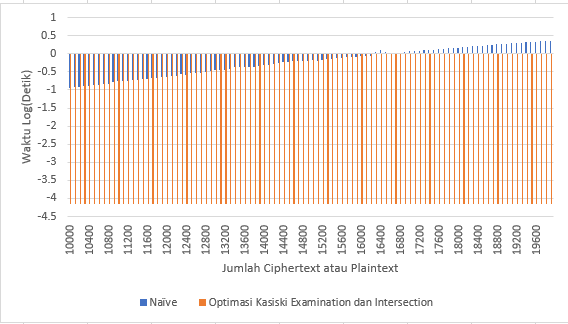
\includegraphics[scale=0.7]{images/bab5/ACD.png}
  	\caption{Gambar Perbandingan Kinerja Algoritma Optimasi \textit{Kasiski Examination} dengan \textit{Intersection} dan \textit{Naive}}
  	\label{fig:banding12}
	\end{figure}
	
	
%telah dilakukan ujicoba apabila menggunakan pure n2 maka tidak akan memungkinkan untuk menyelesaikan masalah ini dengan cepat dan tidak akan berhasil. dilakukan juga untuk membuat perubahan pada intersection akan tetapi juga sesuatu kegagalan. perubahan yang dilakukan untuk mengubah struktur data harus mengakses dengan cepat hanya hal yang mungkin, tapi ini sudah dilakukan . maka yang paling mungkin adalah melakukan optimasi pada pencarian panjang kunci. uji yang telah dilakukan degan menggunakan bilangan prima -> gagal. dengan pigeonhole juga gagal. apbila n=m -> meh podo ae. 
    %\section{Struktur Dokumen \LaTeX{}}
Dokumen \LaTeX{} terdiri dari struktur yang dibuat berdasarkan struktur dokumen sehari-hari. Sebagai penulis dokumen, Anda wajib menggunakan struktur ini sehingga \LaTeX{} dapat melakukan hal lain yang membantu Anda dalam mengorganisir dokumen seperti misalnya pembuatan Daftar Isi. Berikut adalah struktur dokumen yang ada di \LaTeX{} diurutkan berdasarkan hirarkinya.

\begin{ltabulary}{|L|L|} % L = Rata kiri untuk setiap kolom, | = garis batas vertikal.

% Kepala tabel, berulang di setiap halaman
\caption{Struktur hirarki dokumen \LaTeX{}} \label{tabelStrukturDokumen} \\
\hline
\textbf{Nama} & \textbf{Peruntukkan} \\ \hline

\endhead
\endfoot
\endlastfoot

% Isi Tabel
\textbf{\textbackslash{}part\{Judul Bagian\}} & \texttt{book} \\ \hline
\textbf{\textbackslash{}chapter\{Judul Bab\}} & \texttt{book} dan \texttt{report} \\ \hline
\textbf{\textbackslash{}section\{Judul Subbab\}} & semua kecuali \texttt{letter} \\ \hline
\textbf{\textbackslash{}subsection\{Judul Subsubbab\}} & semua kecuali \texttt{letter} \\ \hline
\textbf{\textbackslash{}subsubsection\{Judul Subsubsubbab\}} & semua kecuali \texttt{letter} \\ \hline
\textbf{\textbackslash{}paragraph\{Judul Paragraf\}} & semua\\ \hline

\end{ltabulary}

\subsection{Pengujian Performa}
      Pengujian 
      \subsubsection{Pengujian Kecepatan Fitur A}
      Pengujian fitur ini dilakukan pada lingkungan uji \ref{env_uji1}, dan untuk lebih lengkapnya dapat dilihat pada Tabel \ref{uji1}
      \begin{table}[]
      \centering
      \caption{Pengujian Fitur B}
      \label{uji2}
      \begin{tabular}{llll}
      \multicolumn{1}{c}{\textbf{ID}} & \multicolumn{3}{c}{\textbf{TA-UJI.Proses}}        \\
      Referensi Proses Penggunaan     & \multicolumn{3}{l}{}                              \\
      Nama                            & \multicolumn{3}{l}{}                              \\
      Tujuan Pengujian                & \multicolumn{3}{l}{\multirow{2}{*}{}}             \\
      \textbf{Skenario Pengujian}     & \multicolumn{3}{l}{}                              \\
      Langkah Pengujian               & \multicolumn{3}{l}{}                              \\
      Kecepatan Buka Halaman          & Halaman       & \multicolumn{2}{l}{Google Chrome} \\
                                      & A             & 18 KB           & 0.987s         
      \end{tabular}
      \end{table}
      
    \chapter{PENUTUP}
  Bab ini membahas kesimpulan yang dapat diambil dari tujuan pembuatan sistem dan hubungannya dengan hasil uji coba yang telah dilakukan. Selain itu, terdapat beberapa saran yang bisa dijadikan acuan untuk melakukan pengembangan dan penelitian lebih lanjut.
  \section{Kesimpulan}
 Dari hasil uji coba yang telah dilakukan terhadap perancangan dan implementasi algoritma untuk menyelesaikan SPOJ \textit{The Bytelandian Cryptographer (Act IV)} dapat diambil kesimpulan sebagai berikut:
 
 \begin{enumerate}
 \item Implementasi algoritma dengan menggunakan teknik \textit{Kasiski Examnination} dengan adanya optimasi saja tidak dapat menyelesaikan permasalahan SPOJ \textit{The Bytelandian Cryptographer (Act IV)} dengan benar. Akan tetapi apabila ditambahkan metode \textit{Intersection} didalam teknik \textit{Kasiski Examnination} ditambah dengan optimasi dapat menyelesaikan permasalahan SPOJ \textit{The Bytelandian Cryptographer (Act IV)} dengan benar.
 \item Kompleksitas waktu $\mathcal{O}(T*\frac{M}{2}*(N+S))$ masih dapat menyelesaikan permasalahan SPOJ \textit{The Bytelandian Cryptographer (Act IV)} dalam rentang waktu yang telah ditetapkan.
 \item Waktu yang dibutuhkan oleh program untuk menyelesaikan SPOJ \textit{The Bytelandian Cryptographer (Act IV)} minimum $4,38$ detik, maksimum $4,49$ detik dan rata-rata $4.418$ detik. Memori yang dibutuhkan berkisar antara 26-27 MB. %Dibandingkan dengan menggunakan algoritma \textit{Naive} yang memakan waktu jauh lama. Perbandingannya dapat dilihat pada gambar \ref{fig:banding}.
 \end{enumerate}
  
  \section{Saran}
  Pada Tugas Akhir kali ini tentunya terdapat kekurangan serta nilai-nilai yang dapat penulis ambil. Berikut adalah saran-saran yang dapat diambil melalui Tugas Akhir ini:
  \begin{enumerate}
    \item Teknik \textit{Kasiski Examination} dalam pencarian panjang kunci masih cenderung lambat. Hal ini terjadi karena masih menggunakan teknik \textit{brute force}. Sehingga \textit{running time} yang diperoleh kurang optimal. Perlu adanya optimisasi lanjutan atau penggantian metode yang dapat mencari suatu panjang kunci lebih cepat. Melihat pada Gambar \ref{fig:per1} dan \ref{fig:per2} terdapat yang program yang memiliki \textit{running time} yang lebih cepat.%sebenarnya telah dilakukan ujicoba dengan menggunakan bilangan komposit dan bilangan prima yang telah terbentuk dalam persamaan ini, akan tetapi masih menemukan jalan buntu.
    %\item Perlu adanya Optimisasi dalam hal pencarian suatu indeks yang perlu dirubah atau tidak. Dengan teknik yang dipakai oleh penulis tidak dapat memenuhi ekspetasi jika berharap dengan hasil yang sangat cepat.
    
  \end{enumerate}
  


    % Daftar Pustaka
    %\bibliography{Zotero1}
    %\bibliographystyle{ieeetran}
    
    \appendix % Halaman lampiran, dengan judul LAMPIRAN X
    
 \chapter{Hasil Uji Coba Kebenaran pada Situs SPOJ}
  %\setcounter{figure}{0}
   
   \begin{figure}[H]
   \centering
  	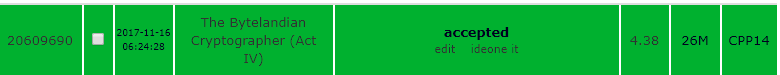
\includegraphics[scale=0.5]{images/lampiran/best.png}
  	\caption{Hasil Uji Coba pada Situs Penilaian SPOJ}
  	\label{fig:best_submission}
  	\end{figure}
	
	 \begin{figure}[H]
  \centering
  	 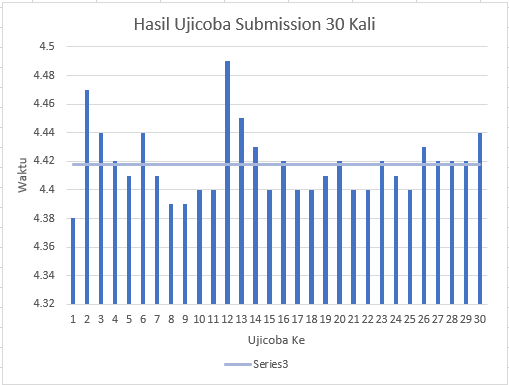
\includegraphics[scale=0.7]{images/lampiran/uji31.png}
  	\caption{Grafik Hasil Uji Coba pada Situs SPOJ Sebanyak 30 Kali}
  	\label{fig:chart}
  \end{figure}  	
  	
  	\begin{figure}[H]
  	\centering
  	 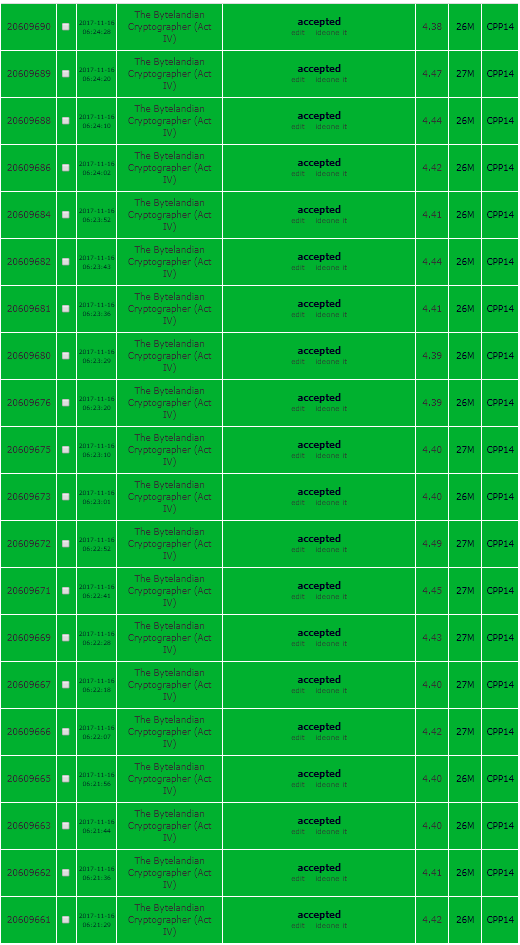
\includegraphics[scale=0.6]{images/lampiran/uji1.png}
  	\caption{Hasil Pengujian Sebanyak 30 Kali pada Situs Penilaian Daring SPOJ (1)}
  	\label{fig:submission1}
  \end{figure}
  
  \begin{figure}[H]
  \centering
  	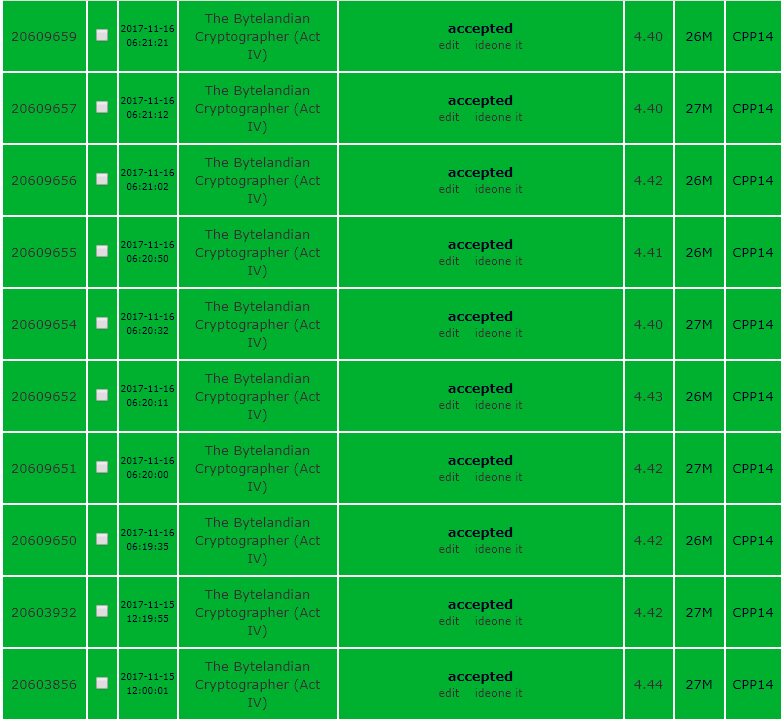
\includegraphics[scale=0.5]{images/lampiran/uji3.png}
  	\caption{Hasil Pengujian Sebanyak 30 Kali pada Situs Penilaian Daring SPOJ (2)}
  	\label{fig:submission2}
  \end{figure}
  
 
  
  

    \chapter{Hasil Percobaan dengan menggunakan Algoritma Naive dan Kasiski Examination}
\setcounter{table}{0}
  \renewcommand{\thetable}{B.\arabic{table}}
  \renewcommand{\thefigure}{B.\arabic{figure}}

\begin{table}[H]
\centering
\caption {Hasil Percobaan Penyelesaian Studi Kasus SPOJ The Bytelandian Cryptographer(Act IV) dengan menggunakan algoritma optimasi \textit{Kasiski Examination} dan \textit{Intersection} (1)}
\begin{tabular}{|c|c|c|}\hline
N&Waktu(Detik)&Waktu(log Detik)\\ \hline
10000&0.0156259&-1.80615\\ \hline
10100&0.0156259&-1.80615\\ \hline
10200&0.0156244&-1.8062\\ \hline
10300&0.0156244&-1.8062\\ \hline
10400&0.0156244&-1.8062\\ \hline
10500&0.0156255&-1.80617\\ \hline
10600&0.0156255&-1.80617\\ \hline
10700&0.0156255&-1.80617\\ \hline
10800&0.0156255&-1.80617\\ \hline
10900&0.0156255&-1.80617\\ \hline
11000&0.0156248&-1.80619\\ \hline
11100&0.0156351&-1.8059\\ \hline
11200&0.0156351&-1.8059\\ \hline
11300&0.0156351&-1.8059\\ \hline
11400&0.0156251&-1.80618\\ \hline
11500&0.0156251&-1.80618\\ \hline
11600&0.0156259&-1.80615\\ \hline
11700&0.0156259&-1.80615\\ \hline
11800&0.0156259&-1.80615\\ \hline
11900&0.0156259&-1.80615\\ \hline
\end{tabular}
\label{tab:res3}
\end{table}
\begin{table}[H]
\centering
\caption {Hasil Percobaan Penyelesaian Studi Kasus SPOJ The Bytelandian Cryptographer(Act IV) dengan menggunakan algoritma optimasi \textit{Kasiski Examination} dan \textit{Intersection} (2)}
\begin{tabular}{|c|c|c|}\hline
N&Waktu(Detik)&Waktu(log Detik)\\ \hline
12000&0.0156252&-1.80617\\ \hline
12100&0.0156252&-1.80617\\ \hline
12200&0.001048&-2.97964\\ \hline
12300&0.0156267&-1.80613\\ \hline
12400&0.0156267&-1.80613\\ \hline
12500&0.0156267&-1.80613\\ \hline
12600&0.0156237&-1.80622\\ \hline
12700&0.0156237&-1.80622\\ \hline
12800&0.0156244&-1.8062\\ \hline
12900&0.0156244&-1.8062\\ \hline
13000&0.0156244&-1.8062\\ \hline
13100&0.0156244&-1.8062\\ \hline
13200&0.0156244&-1.8062\\ \hline
13300&0.0156244&-1.8062\\ \hline
13400&0.0156229&-1.80624\\ \hline
13500&0.0156251&-1.80618\\ \hline
13600&0.0156441&-1.80565\\ \hline
13700&0.0156351&-1.8059\\ \hline
13800&0.0156351&-1.8059\\ \hline
13900&0.0156351&-1.8059\\ \hline
\end{tabular}
\label{tab:res5}
\end{table}
\begin{table}[H]
\centering
\caption {Hasil Percobaan Penyelesaian Studi Kasus SPOJ The Bytelandian Cryptographer(Act IV) dengan menggunakan algoritma optimasi \textit{Kasiski Examination} dan \textit{Intersection} (3)}
\begin{tabular}{|c|c|c|}\hline
N&Waktu(Detik)&Waktu(log Detik)\\ \hline
14000&0.0156149&-1.80646\\ \hline
14100&0.0156252&-1.80617\\ \hline
14200&0.0156252&-1.80617\\ \hline
14300&0.0156252&-1.80617\\ \hline
14400&0.0156343&-1.80592\\ \hline
14500&0.0156343&-1.80592\\ \hline
14600&0.0156343&-1.80592\\ \hline
14700&0.0156343&-1.80592\\ \hline
14800&0.0156229&-1.80624\\ \hline
14900&0.0156229&-1.80624\\ \hline
15000&0.0156229&-1.80624\\ \hline
15100&0.0156229&-1.80624\\ \hline
15200&0.0156229&-1.80624\\ \hline
15300&0.0156229&-1.80624\\ \hline
15400&0.0156354&-1.80589\\ \hline
15500&0.0156263&-1.80614\\ \hline
15600&0.0156263&-1.80614\\ \hline
15700&0.0156263&-1.80614\\ \hline
15800&0.0156263&-1.80614\\ \hline
15900&0.0156278&-1.8061\\ \hline
\end{tabular}
\label{tab:res7}
\end{table}
\begin{table}[H]
\centering
\caption {Hasil Percobaan Penyelesaian Studi Kasus SPOJ The Bytelandian Cryptographer(Act IV) dengan menggunakan algoritma optimasi \textit{Kasiski Examination} dan \textit{Intersection} (4)}
\begin{tabular}{|c|c|c|}\hline
N&Waktu(Detik)&Waktu(log Detik)\\ \hline
16000&0.0156256&-1.80616\\ \hline
16100&0.0156256&-1.80616\\ \hline
16200&0.0156256&-1.80616\\ \hline
16300&0.0156351&-1.8059\\ \hline
16400&0.0156244&-1.8062\\ \hline
16500&0.0156278&-1.8061\\ \hline
16600&0.0156278&-1.8061\\ \hline
16700&0.0156278&-1.8061\\ \hline
16800&0.0227098&-1.64379\\ \hline
16900&0.0156351&-1.8059\\ \hline
17000&0.0156153&-1.80645\\ \hline
17100&0.0156153&-1.80645\\ \hline
17200&0.0156153&-1.80645\\ \hline
17300&0.015635&-1.8059\\ \hline
17400&0.0156259&-1.80615\\ \hline
17500&0.0156347&-1.80591\\ \hline
17600&0.0156153&-1.80645\\ \hline
17700&0.0156153&-1.80645\\ \hline
17800&0.0156191&-1.80634\\ \hline
17900&0.0156247&-1.80619\\ \hline
\end{tabular}
\label{tab:res9}
\end{table}
\begin{table}[H]
\centering
\caption {Hasil Percobaan Penyelesaian Studi Kasus SPOJ The Bytelandian Cryptographer(Act IV) dengan menggunakan algoritma optimasi \textit{Kasiski Examination} dan \textit{Intersection} (5)}
\begin{tabular}{|c|c|c|}\hline
N&Waktu(Detik)&Waktu(log Detik)\\ \hline
18000&0.0156247&-1.80619\\ \hline
18100&0.0156247&-1.80619\\ \hline
18200&0.0156247&-1.80619\\ \hline
18300&0.0156229&-1.80624\\ \hline
18400&0.0156255&-1.80617\\ \hline
18500&0.0156247&-1.80619\\ \hline
18600&0.0156225&-1.80625\\ \hline
18700&0.0156225&-1.80625\\ \hline
18800&0.0156225&-1.80625\\ \hline
18900&0.0156225&-1.80625\\ \hline
19000&0.0156248&-1.80619\\ \hline
19100&0.0156275&-1.80611\\ \hline
19200&0.0156252&-1.80617\\ \hline
19300&0.0156206&-1.8063\\ \hline
19400&0.015626&-1.80615\\ \hline
19500&0.015626&-1.80615\\ \hline
19600&0.015626&-1.80615\\ \hline
19700&0.015626&-1.80615\\ \hline
19800&0.015626&-1.80615\\ \hline
19900&0.0156248&-1.80619\\ \hline
\end{tabular}
\label{tab:res11}
\end{table}


\begin{table}[H]
\centering
\caption {Hasil Percobaan Penyelesaian Studi Kasus SPOJ The Bytelandian Cryptographer(Act IV) dengan menggunakan algoritma \textit{Naive} (1)}
\begin{tabular}{|c|c|c|}\hline
N&Waktu(Detik)&Waktu(log Detik)\\ \hline
10000&0.390619\\ \hline
10100&0.394834\\ \hline
10200&0.400778\\ \hline
10300&0.406246\\ \hline
10400&0.406737\\ \hline
10500&0.42187\\ \hline
10600&0.421361\\ \hline
10700&0.437496\\ \hline
10800&0.437661\\ \hline
10900&0.45313\\ \hline
11000&0.468254\\ \hline
11100&0.468746\\ \hline
11200&0.469241\\ \hline
11300&0.48438\\ \hline
11400&0.48388\\ \hline
11500&0.498918\\ \hline
11600&0.501698\\ \hline
11700&0.515621\\ \hline
11800&0.516122\\ \hline
11900&0.531256\\ \hline
\end{tabular}
\label{tab:res2}
\end{table}
\begin{table}[H]
\centering
\caption {Hasil Percobaan Penyelesaian Studi Kasus SPOJ The Bytelandian Cryptographer(Act IV) dengan menggunakan algoritma \textit{Naive} (2)}
\begin{tabular}{|c|c|c|}\hline
N&Waktu(Detik)&Waktu(log Detik)\\ \hline
12000&0.530714\\ \hline
12100&0.546407\\ \hline
12200&0.54688\\ \hline
12300&0.578888\\ \hline
12400&0.562516\\ \hline
12500&0.593242\\ \hline
12600&0.594233\\ \hline
12700&0.593746\\ \hline
12800&0.608855\\ \hline
12900&0.621452\\ \hline
13000&0.640633\\ \hline
13100&0.640096\\ \hline
13200&0.641099\\ \hline
13300&0.656247\\ \hline
13400&0.687057\\ \hline
13500&0.687981\\ \hline
13600&0.687508\\ \hline
13700&0.702599\\ \hline
13800&0.703614\\ \hline
13900&0.718225\\ \hline
\end{tabular}
\label{tab:res4}
\end{table}
\begin{table}[H]
\centering
\caption {Hasil Percobaan Penyelesaian Studi Kasus SPOJ The Bytelandian Cryptographer(Act IV) dengan menggunakan algoritma \textit{Naive} (3)}
\begin{tabular}{|c|c|c|}\hline
N&Waktu(Detik)&Waktu(log Detik)\\ \hline
14000&0.734383\\ \hline
14100&0.734832\\ \hline
14200&0.749211\\ \hline
14300&0.766334\\ \hline
14400&0.789337\\ \hline
14500&0.796879\\ \hline
14600&0.81308\\ \hline
14700&0.812038\\ \hline
14800&0.813018\\ \hline
14900&0.827625\\ \hline
15000&0.844241\\ \hline
15100&0.827581\\ \hline
15200&0.843761\\ \hline
15300&0.859857\\ \hline
15400&0.874509\\ \hline
15500&0.891106\\ \hline
15600&0.890121\\ \hline
15700&0.906285\\ \hline
15800&0.921589\\ \hline
15900&0.922729\\ \hline
\end{tabular}
\label{tab:res6}
\end{table}
\begin{table}[H]
\centering
\caption {Hasil Percobaan Penyelesaian Studi Kasus SPOJ The Bytelandian Cryptographer(Act IV) dengan menggunakan algoritma \textit{Naive} (4)}
\begin{tabular}{|c|c|c|}\hline
N&Waktu(Detik)&Waktu(log Detik)\\ \hline
16000&0.937003\\ \hline
16100&0.952834\\ \hline
16200&0.953624\\ \hline
16300&1.04645\\ \hline
16400&1.10416\\ \hline
16500&1.0375\\ \hline
16600&1.03005\\ \hline
16700&1.03179\\ \hline
16800&1.03075\\ \hline
16900&1.04765\\ \hline
17000&1.07823\\ \hline
17100&1.09324\\ \hline
17200&1.09423\\ \hline
17300&1.10882\\ \hline
17400&1.10902\\ \hline
17500&1.12558\\ \hline
17600&1.14016\\ \hline
17700&1.15626\\ \hline
17800&1.17237\\ \hline
17900&1.18701\\ \hline
\end{tabular}
\label{tab:res8}
\end{table}
\begin{table}[H]
\centering
\caption {Hasil Percobaan Penyelesaian Studi Kasus SPOJ The Bytelandian Cryptographer(Act IV) dengan menggunakan algoritma \textit{Naive} (5)}
\begin{tabular}{|c|c|c|}\hline
N&Waktu(Detik)&Waktu(log Detik)\\ \hline
18000&1.18803\\ \hline
18100&1.20266\\ \hline
18200&1.21944\\ \hline
18300&1.23395\\ \hline
18400&1.24748\\ \hline
18500&1.25243\\ \hline
18600&1.26614\\ \hline
18700&1.28063\\ \hline
18800&1.2969\\ \hline
18900&1.31404\\ \hline
19000&1.32662\\ \hline
19100&1.35917\\ \hline
19200&1.34388\\ \hline
19300&1.36163\\ \hline
19400&1.37299\\ \hline
19500&1.39379\\ \hline
19600&1.40303\\ \hline
19700&1.43746\\ \hline
19800&1.43739\\ \hline
19900&1.43803\\ \hline
\end{tabular}
\label{tab:res10}
\end{table}
  \backmatter % Lampiran tanpa judul LAMPIRAN X, untuk BIODATA PENULIS

   \chapter{BIODATA PENULIS}
		\begin{wrapfigure}{l}{0.3\textwidth}
			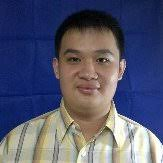
\includegraphics[width=0.3\textwidth]{images/foto-diri.jpg}
		\end{wrapfigure}
		\textbf{\ \\Freddy Hermawan Yuwono}, kelahiran \& besar di Bondowoso-Jawa Timur, sangat suka membaca. Penulis menempuh jenjang pendidikan S1 Teknik Informatika ITS dari tahun 2013 sampai dengan dibuatnya buku ini.\\
		
		\indent Motto penulis yaitu "Segala sesuatu pasti akan terjadi dan pasti akan dilewati", membawa penulis mencoba belajar yang baru topik tugas akhir ini, dimana penulis dapat menerapkan sesuatu yang belum pernah penulis untuk melaluinya. Algoritma, optimasi dan pelajaran yang penulis petik dari yang pernah dilakukan oleh penulis sebelumnya, dengan bimbingan dosen-dosen pembimbing. Dalam pendalaman topik tugas akhir ini juga, penulis banyak belajar dan menjadi sangat tertarik mendalami \textit{cryptography}, dan \textit{data scientist \& engineering}. \\
		\indent Dengan segala kerendahan hati, ilmu penulis masihlah setitik dibandingkan susu sebelanga. Penulis sangat mengharapkan diskusi, ajaran dan bantuan dalam memperbaiki diri. Apabila pembaca berkenan, penulis dapat dihubungi melalui \textit{email} ke \texttt{freddy.yuwono@gmail.com}.



\end{document}